\documentclass[aspectratio=169,10pt]{beamer}
\usetheme{metropolis}
\usecolortheme{default}
\definecolor{primaryblue}{RGB}{20,75,140}
\definecolor{secondaryblue}{RGB}{70,130,180}
\definecolor{accentorange}{RGB}{230,95,45}

\usepackage{amsmath}
\usepackage{amssymb}
\usepackage{graphicx}
\usepackage{booktabs}
\usepackage{algorithm}
\usepackage{algorithmic}

% Title information
\title{Feature Extraction and Representation}
\subtitle{CMSC 178IP - Digital Image Processing}
\author{Noel Jeffrey Pinton}
\institute{University of the Philippines - Cebu\\Department of Computer Science}
\date{}

\begin{document}

\maketitle

% Introduction Section
\section{Introduction}

\begin{frame}{What is Feature Extraction?}
    \begin{alertblock}{Definition}
        Feature extraction transforms raw image data into a reduced representation that captures the most relevant information for a specific task.
    \end{alertblock}

    \begin{columns}[c]
        \begin{column}{0.5\textwidth}
            \textbf{Key Objectives:}
            \begin{itemize}
                \item Reduce dimensionality
                \item Extract meaningful patterns
                \item Enable robust matching
                \item Facilitate recognition tasks
            \end{itemize}
        \end{column}
        \begin{column}{0.5\textwidth}
            \textbf{Applications:}
            \begin{itemize}
                \item Object recognition
                \item Image registration
                \item Medical imaging
                \item Quality inspection
            \end{itemize}
        \end{column}
    \end{columns}
\end{frame}

\begin{frame}{Types of Image Features}
    \begin{columns}[c]
        \begin{column}{0.33\textwidth}
            \textbf{Low-Level Features}
            \begin{itemize}
                \item Edges and boundaries
                \item Corners and keypoints
                \item Textures and patterns
                \item Color distributions
            \end{itemize}
        \end{column}
        \begin{column}{0.33\textwidth}
            \textbf{Mid-Level Features}
            \begin{itemize}
                \item Shape descriptors
                \item Region properties
                \item Spatial relationships
                \item Local patterns
            \end{itemize}
        \end{column}
        \begin{column}{0.33\textwidth}
            \textbf{High-Level Features}
            \begin{itemize}
                \item Object parts
                \item Semantic concepts
                \item Scene understanding
                \item Context information
            \end{itemize}
        \end{column}
    \end{columns}
\end{frame}

% Edge and Line Detection Section
\section{Edge and Line Detection}

\begin{frame}{Edge Detection: Mathematical Foundation}
    \begin{alertblock}{Edge Definition}
        An edge represents a significant local change in image intensity, typically occurring at object boundaries.
    \end{alertblock}

    \textbf{Gradient-Based Approach:}
    \begin{align}
        \nabla I &= \left[\frac{\partial I}{\partial x}, \frac{\partial I}{\partial y}\right]^T \\
        |\nabla I| &= \sqrt{\left(\frac{\partial I}{\partial x}\right)^2 + \left(\frac{\partial I}{\partial y}\right)^2} \\
        \theta &= \arctan\left(\frac{\partial I/\partial y}{\partial I/\partial x}\right)
    \end{align}

    Where $|\nabla I|$ is the gradient magnitude and $\theta$ is the gradient direction.
\end{frame}

\begin{frame}{Gradient Operators}
    \begin{center}
        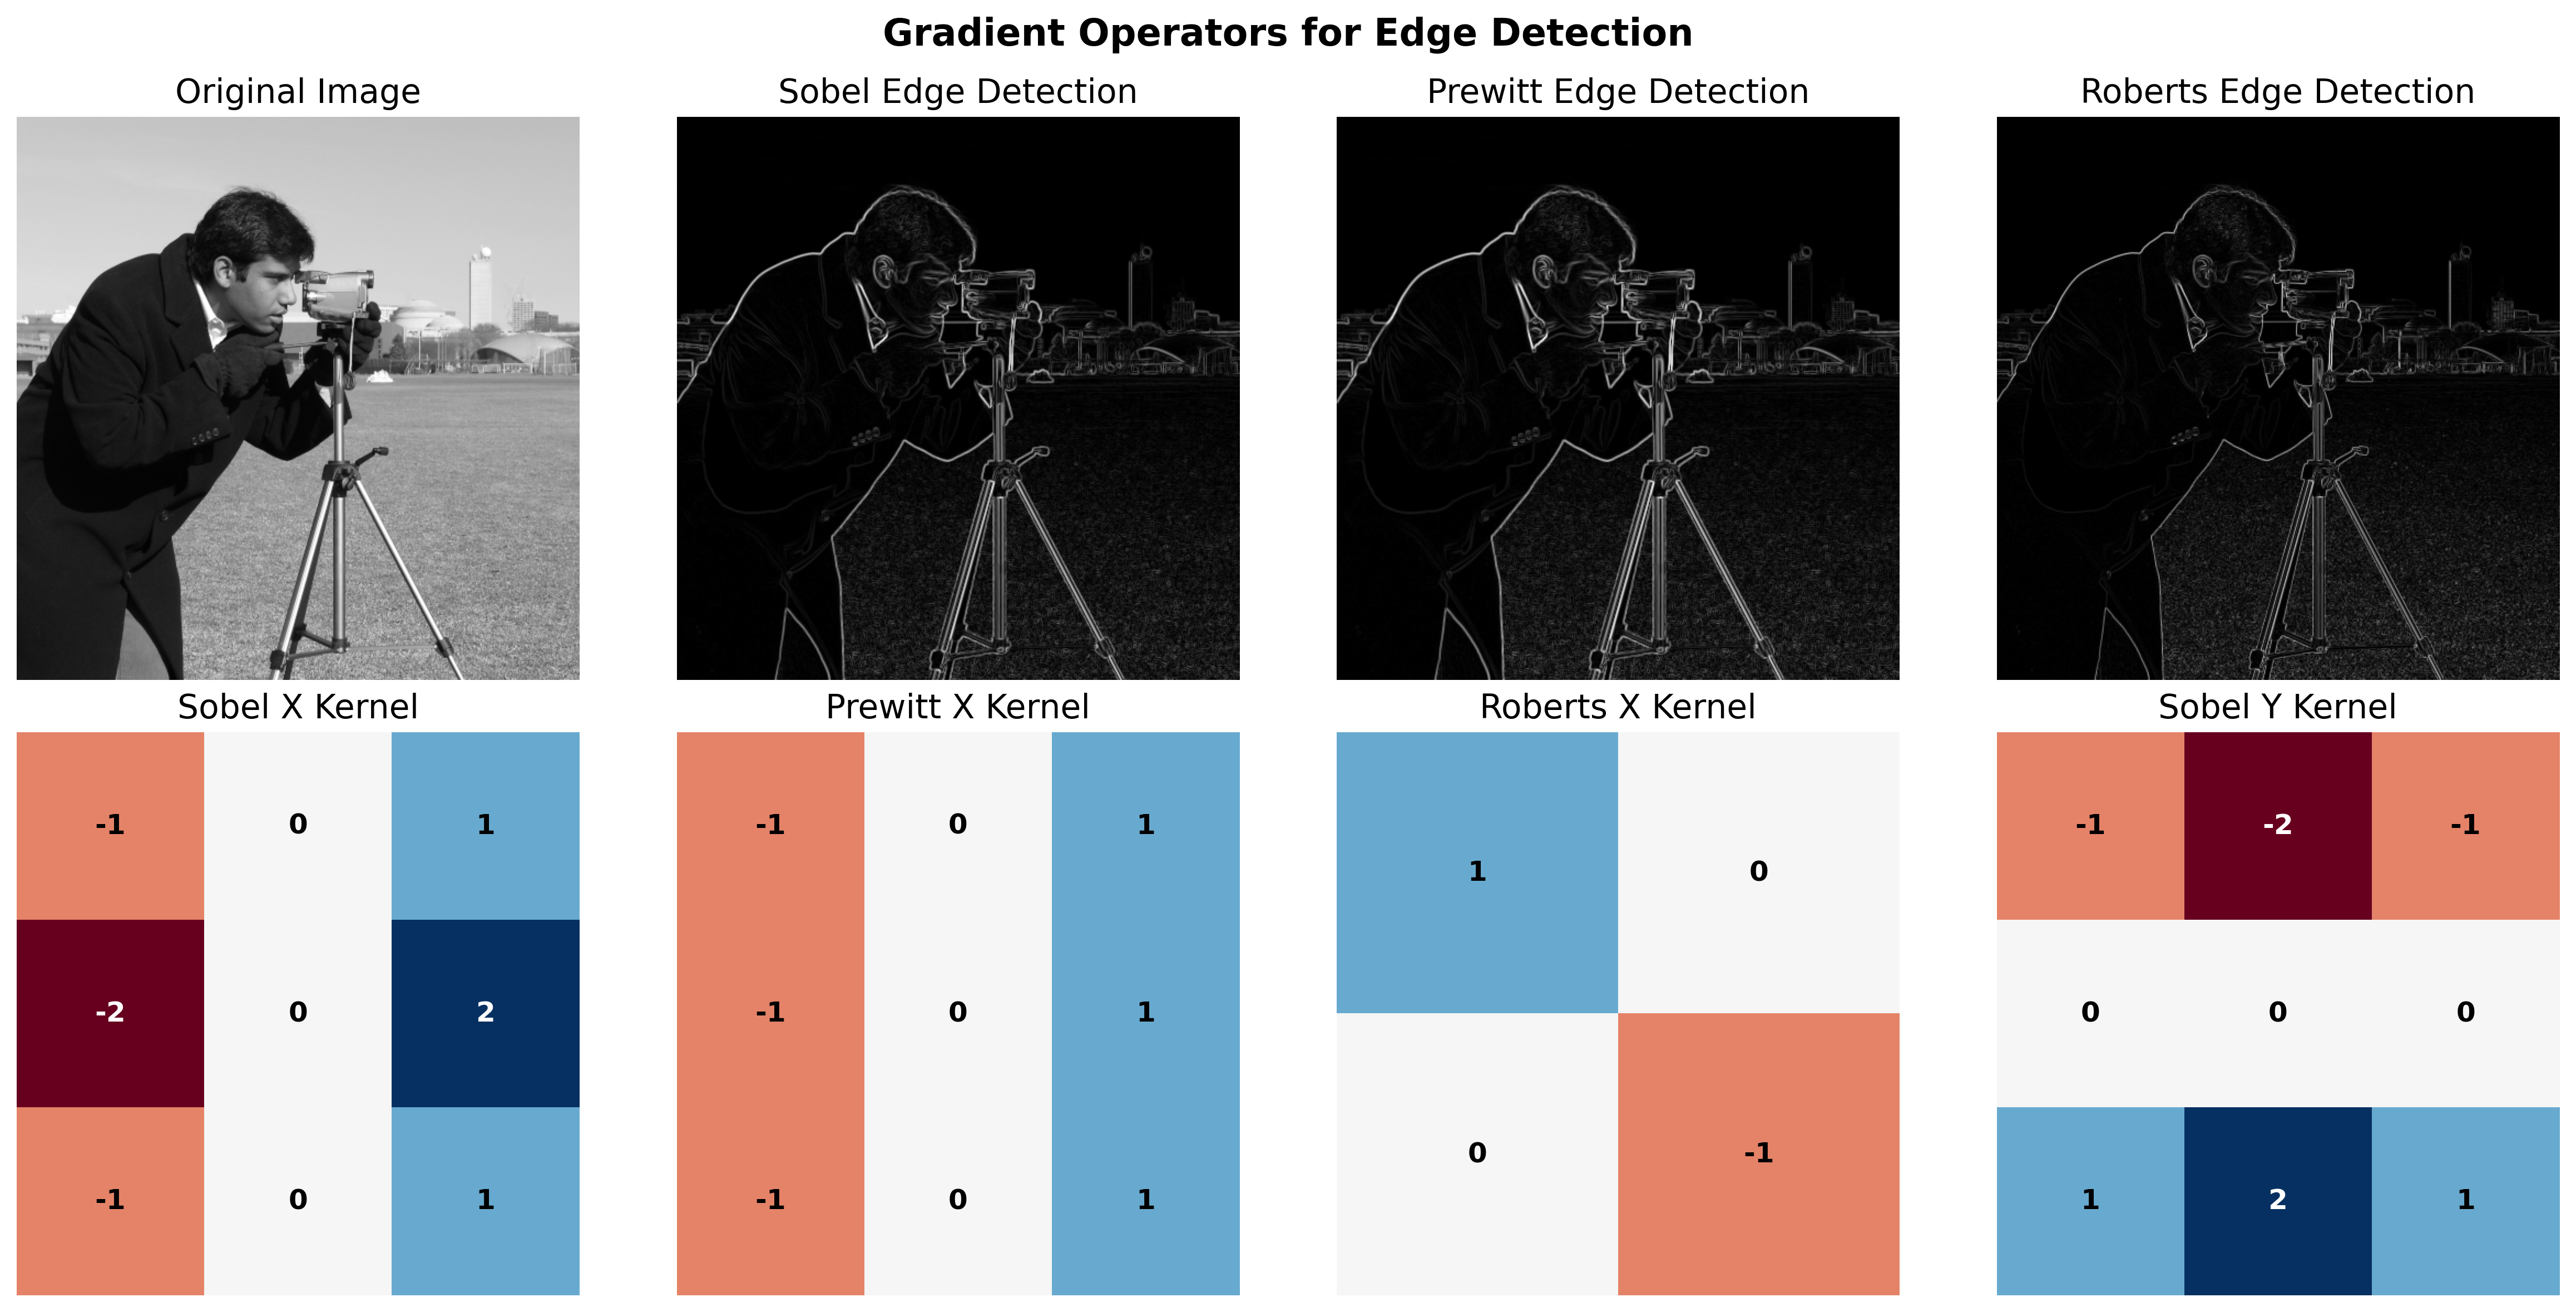
\includegraphics[width=0.85\textwidth,height=0.65\textheight,keepaspectratio]{../figures/gradient_operators.png}
    \end{center}

    \begin{columns}[c]
        \begin{column}{0.5\textwidth}
            \textbf{Sobel Operator:}
            \begin{itemize}
                \item Combines Gaussian smoothing
                \item Good noise suppression
                \item Most commonly used
            \end{itemize}
        \end{column}
        \begin{column}{0.5\textwidth}
            \textbf{Key Properties:}
            \begin{itemize}
                \item Separable convolution
                \item Directional sensitivity
                \item Computational efficiency
            \end{itemize}
        \end{column}
    \end{columns}
\end{frame}

\begin{frame}{Edge Detection Methods Comparison}
    \begin{center}
        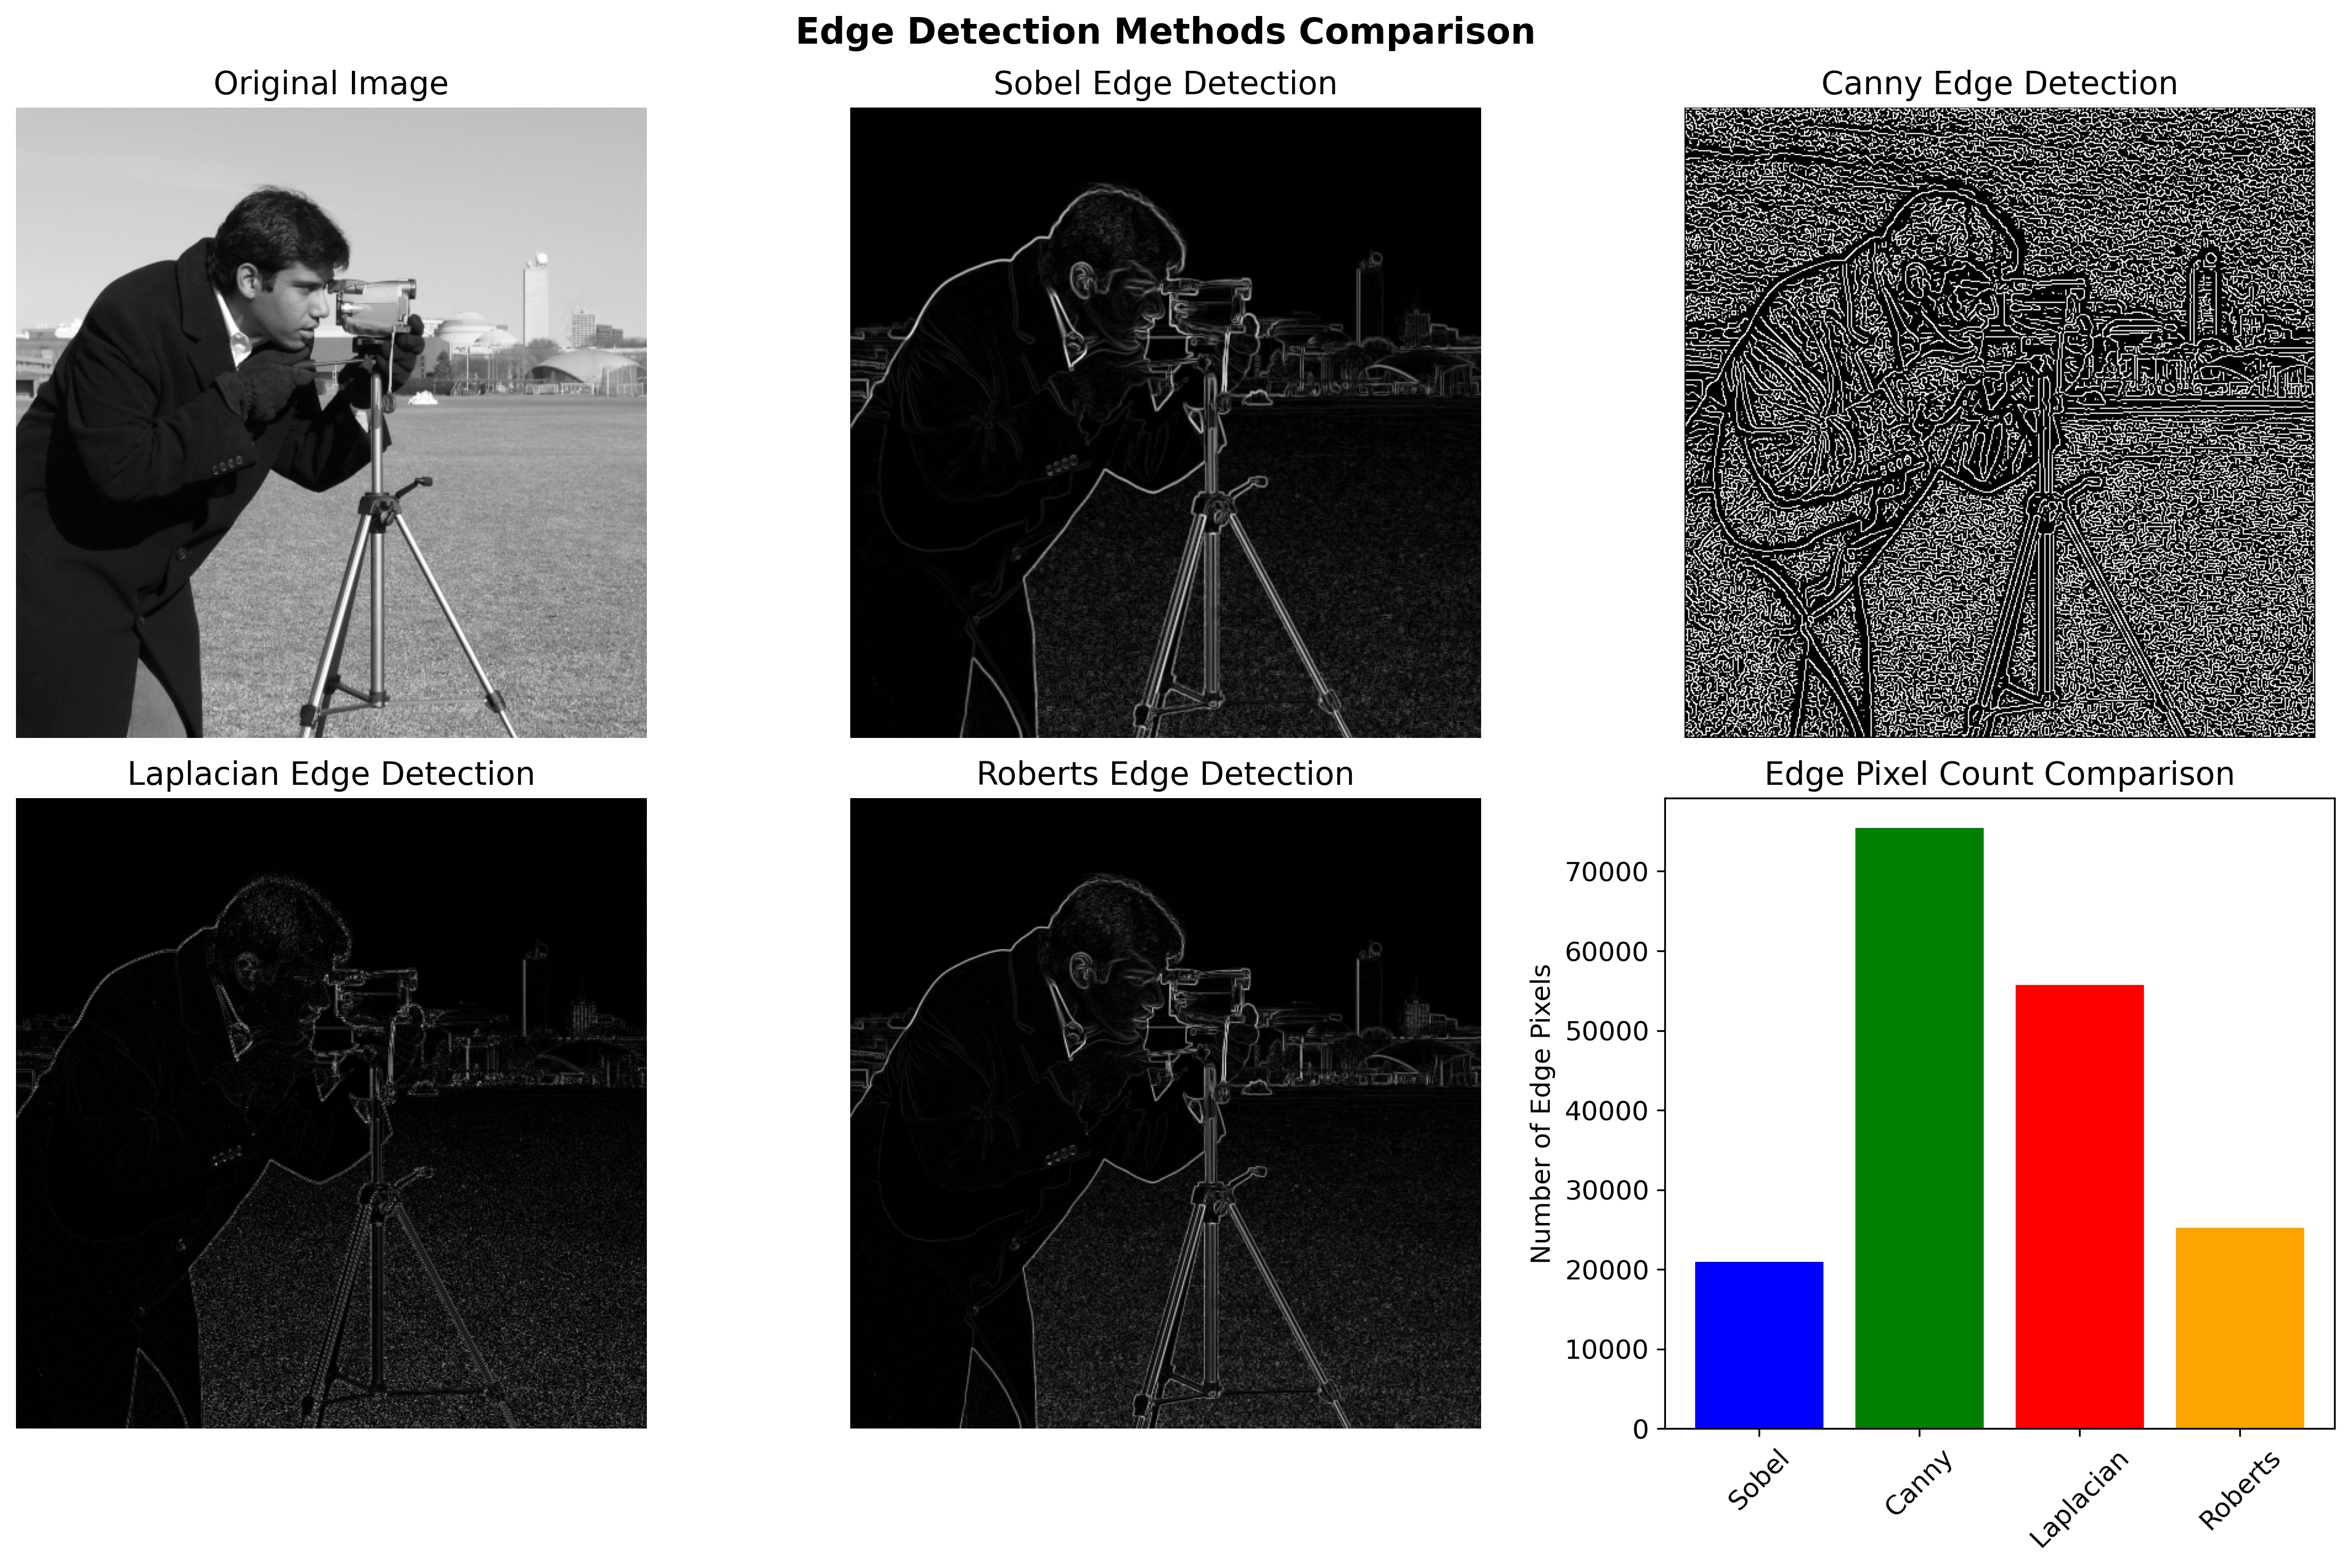
\includegraphics[width=0.8\textwidth,height=0.6\textheight,keepaspectratio]{../figures/edge_detection_comparison.png}
    \end{center}
\end{frame}

\begin{frame}{Canny Edge Detector Details}
    \begin{columns}[c]
        \begin{column}{0.5\textwidth}
            \textbf{Canny Edge Detector:}
            \begin{itemize}
                \item Multi-stage algorithm
                \item Non-maximum suppression
                \item Double thresholding
                \item Edge linking by hysteresis
            \end{itemize}
        \end{column}
        \begin{column}{0.5\textwidth}
            \textbf{Advantages:}
            \begin{itemize}
                \item Low error rate
                \item Good localization
                \item Single response to edges
                \item Optimal edge detection
            \end{itemize}
        \end{column}
    \end{columns}
\end{frame}

\begin{frame}{Canny Edge Detection Algorithm}
    \begin{algorithm}[H]
        \begin{algorithmic}[1]
            \STATE Apply Gaussian filter to smooth the image
            \STATE Compute intensity gradients using Sobel operator
            \STATE Apply non-maximum suppression to thin edges
            \STATE Apply double threshold to determine potential edges
            \STATE Track edges by hysteresis: suppress weak edges not connected to strong edges
        \end{algorithmic}
    \end{algorithm}

    \begin{alertblock}{Key Parameters}
        \begin{itemize}
            \item $\sigma$: Gaussian smoothing parameter
            \item $T_{high}$: High threshold for strong edges
            \item $T_{low}$: Low threshold for weak edges (typically $T_{low} = 0.4 \times T_{high}$)
        \end{itemize}
    \end{alertblock}
\end{frame}

\begin{frame}{Hough Transform for Line Detection}
    \begin{center}
        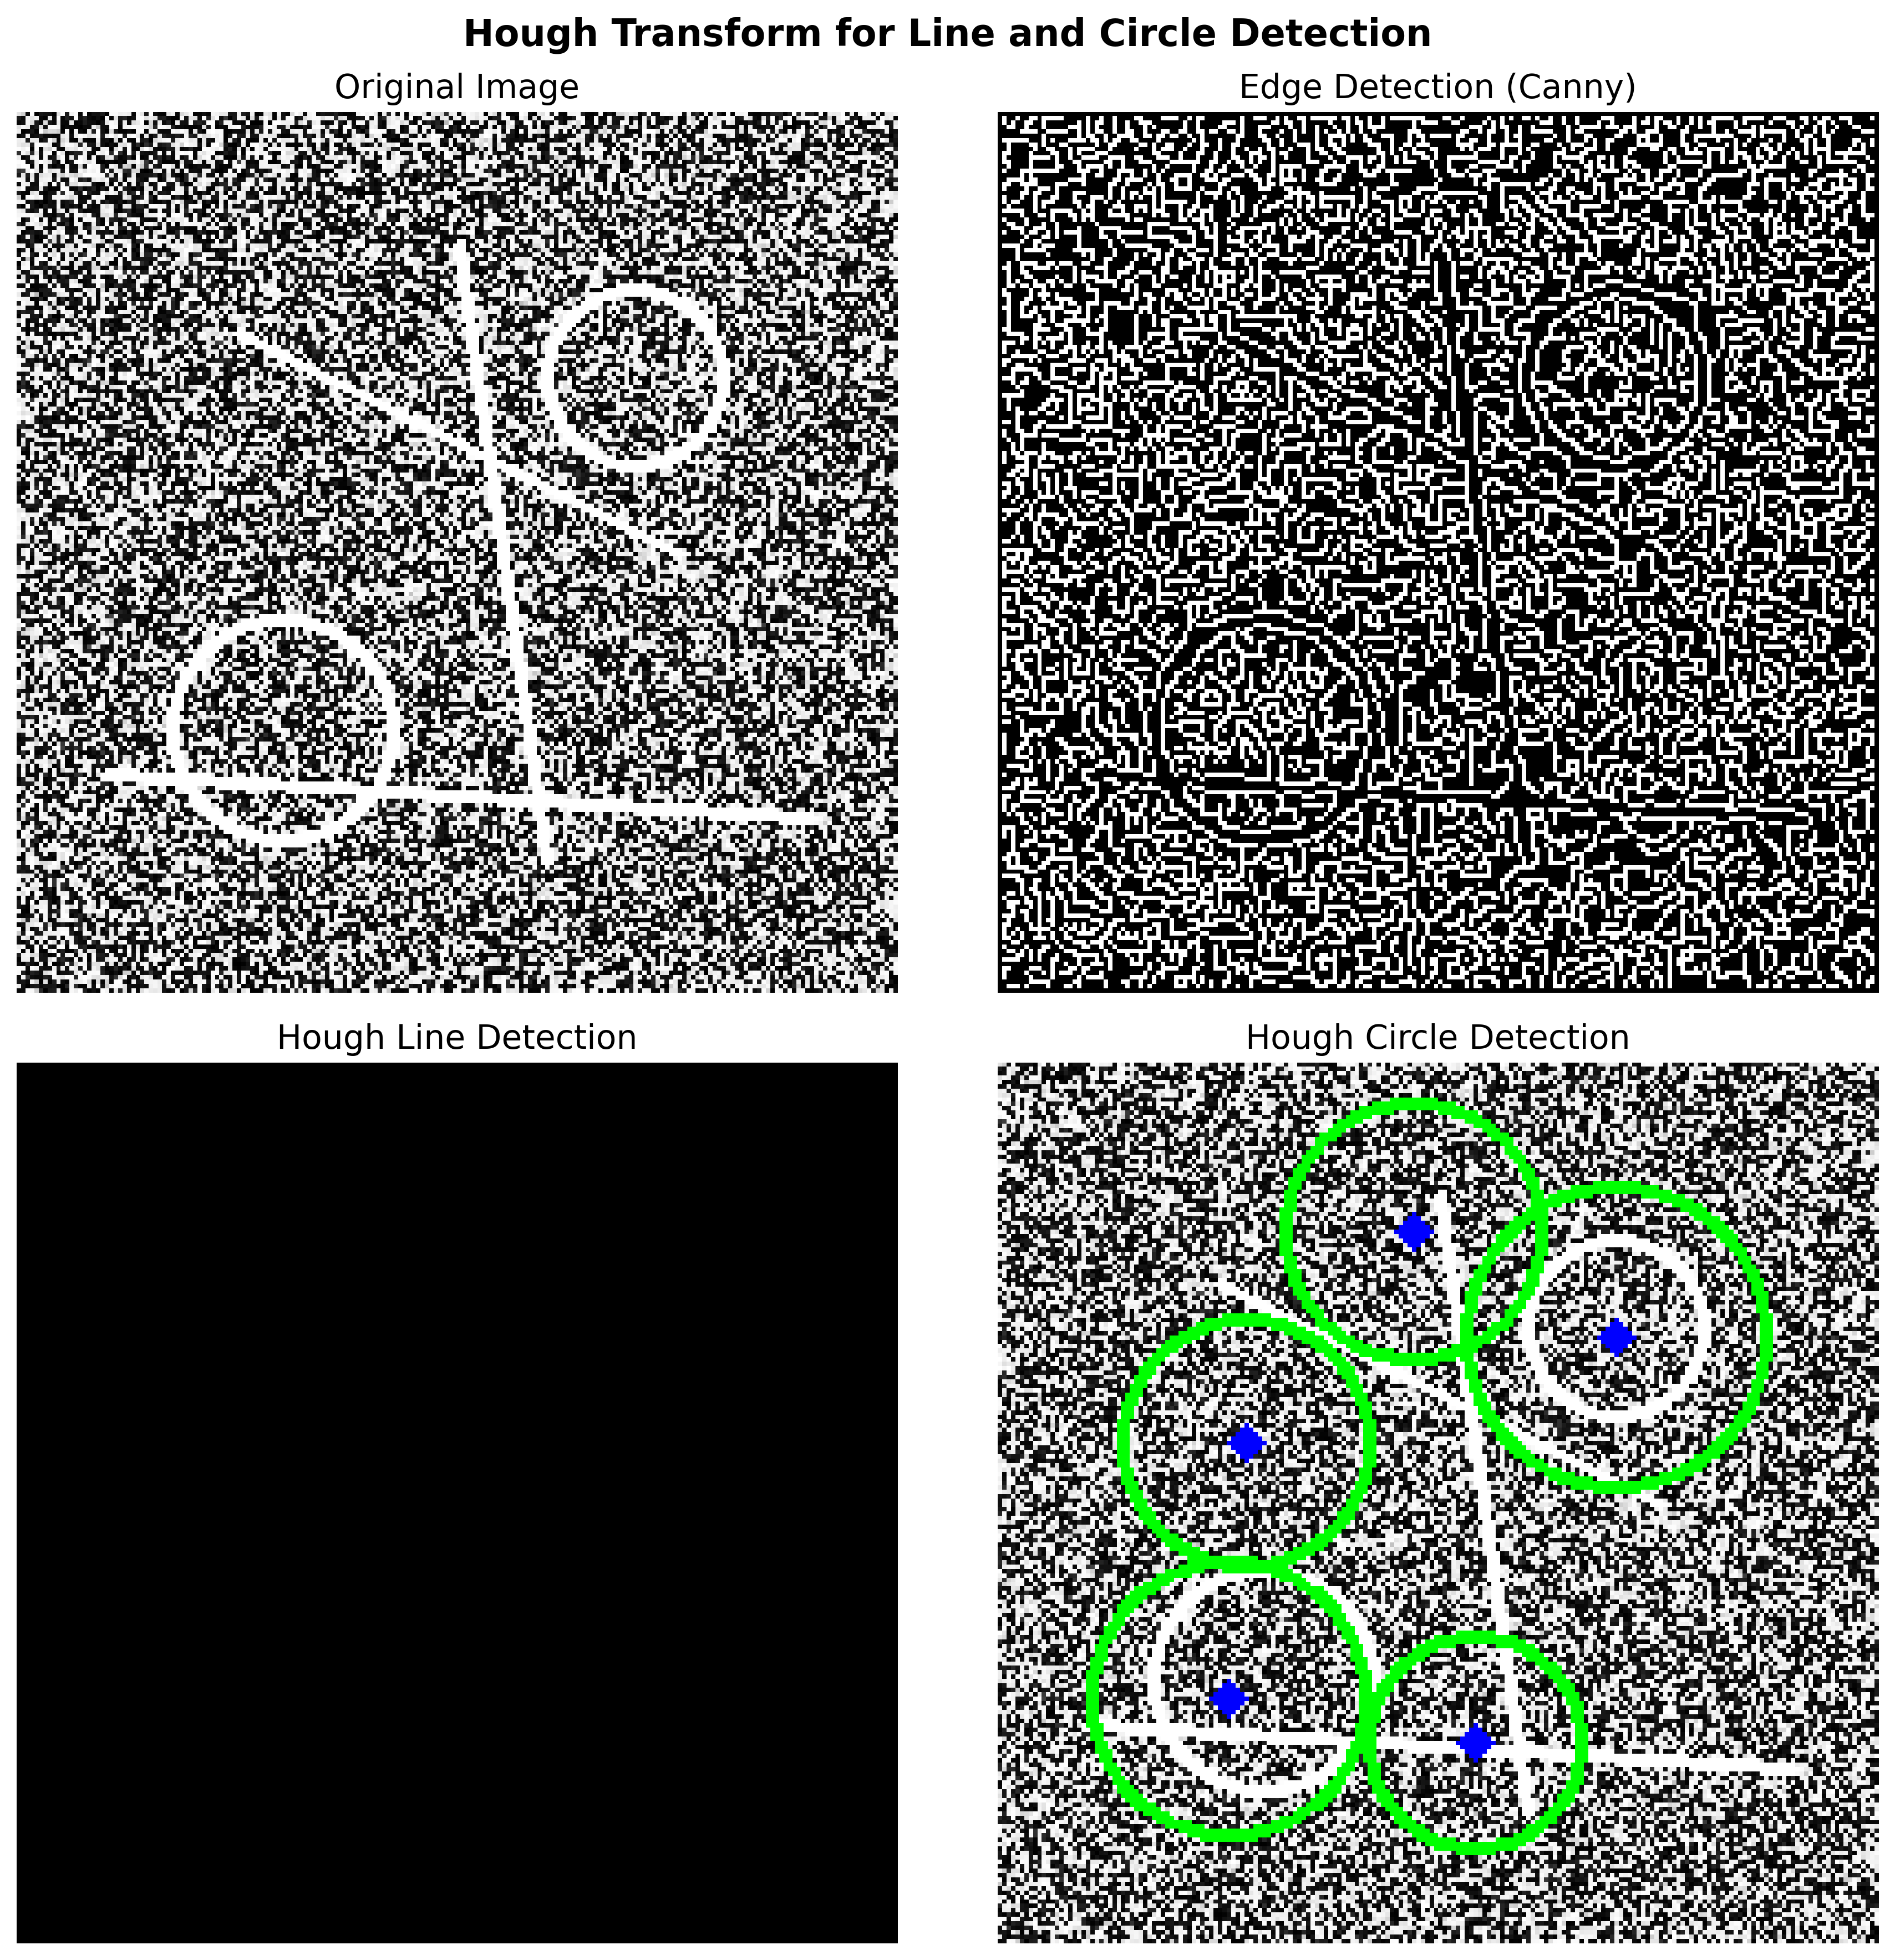
\includegraphics[width=0.7\textwidth,height=0.5\textheight,keepaspectratio]{../figures/hough_transform_demo.png}
    \end{center}

    \textbf{Parametric Representation:}
    \begin{align}
        \rho &= x \cos\theta + y \sin\theta
    \end{align}

    Where $\rho$ is distance from origin, $\theta$ is angle of normal.
\end{frame}

\begin{frame}{Hough Transform: Mathematical Principle}
    \begin{columns}[c]
        \begin{column}{0.6\textwidth}
            \textbf{Algorithm Steps:}
            \begin{enumerate}
                \item Convert image to edge map
                \item For each edge pixel $(x_i, y_i)$:
                \begin{itemize}
                    \item For $\theta = 0$ to $180^\circ$
                    \item Calculate $\rho = x_i \cos\theta + y_i \sin\theta$
                    \item Increment accumulator $A(\rho, \theta)$
                \end{itemize}
                \item Find peaks in accumulator array
                \item Extract line parameters from peaks
            \end{enumerate}
        \end{column}
        \begin{column}{0.4\textwidth}
            \textbf{Advantages:}
            \begin{itemize}
                \item Robust to noise
                \item Handles partial occlusion
                \item Globally optimal
                \item Parameter estimation
            \end{itemize}

            \textbf{Limitations:}
            \begin{itemize}
                \item Computational complexity
                \item Memory requirements
                \item Peak detection challenges
            \end{itemize}
        \end{column}
    \end{columns}
\end{frame}

% Texture and Local Features Section
\section{Texture and Local Features}

\begin{frame}{Texture Analysis Fundamentals}
    \begin{alertblock}{Texture Definition}
        Texture describes the spatial arrangement of intensity variations in an image region, characterized by patterns, regularity, and statistical properties.
    \end{alertblock}

    \begin{center}
        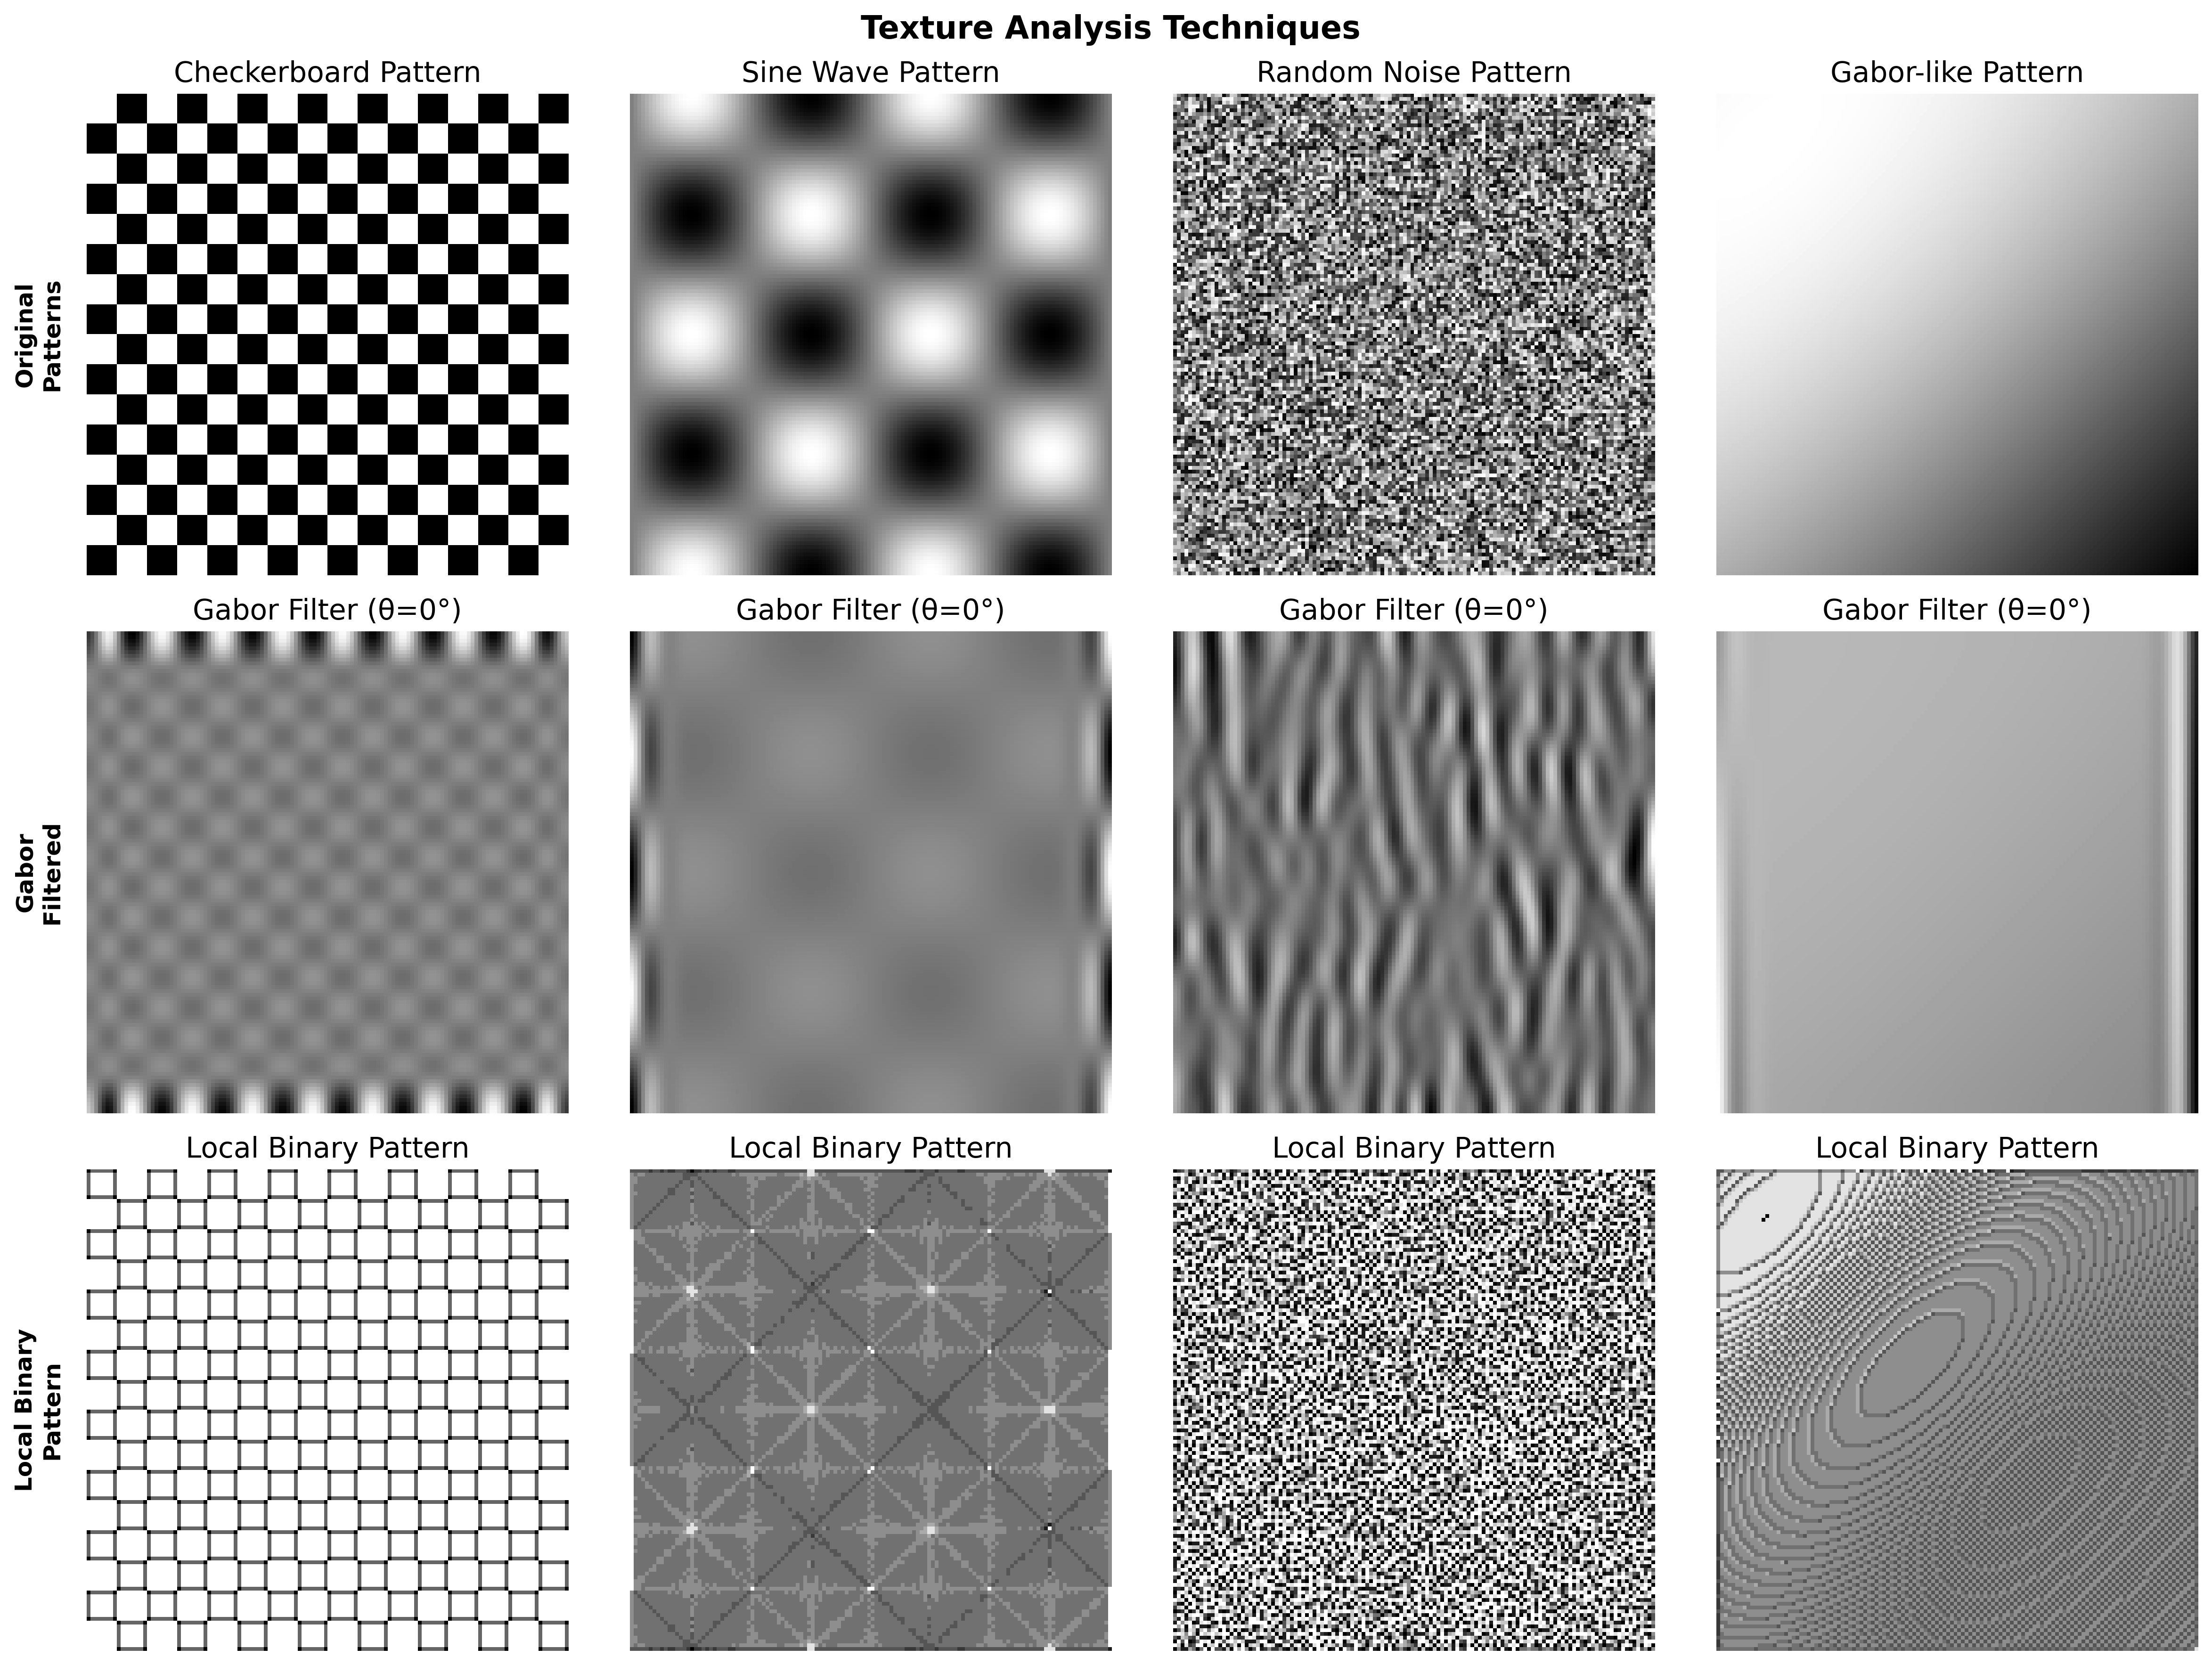
\includegraphics[width=0.75\textwidth,height=0.6\textheight,keepaspectratio]{../figures/texture_analysis.png}
    \end{center}
\end{frame}

\begin{frame}{Local Binary Patterns (LBP)}
    \textbf{Mathematical Definition:}
    \begin{align}
        LBP_{P,R}(x_c, y_c) &= \sum_{p=0}^{P-1} s(g_p - g_c) \cdot 2^p \\
        s(x) &= \begin{cases}
            1 & \text{if } x \geq 0 \\
            0 & \text{if } x < 0
        \end{cases}
    \end{align}

    Where:
    \begin{itemize}
        \item $g_c$ is the intensity of the center pixel
        \item $g_p$ is the intensity of the $p$-th neighbor
        \item $P$ is the number of sampling points
        \item $R$ is the radius of the sampling circle
    \end{itemize}
\end{frame}

\begin{frame}{Advanced LBP Analysis}
    \begin{center}
        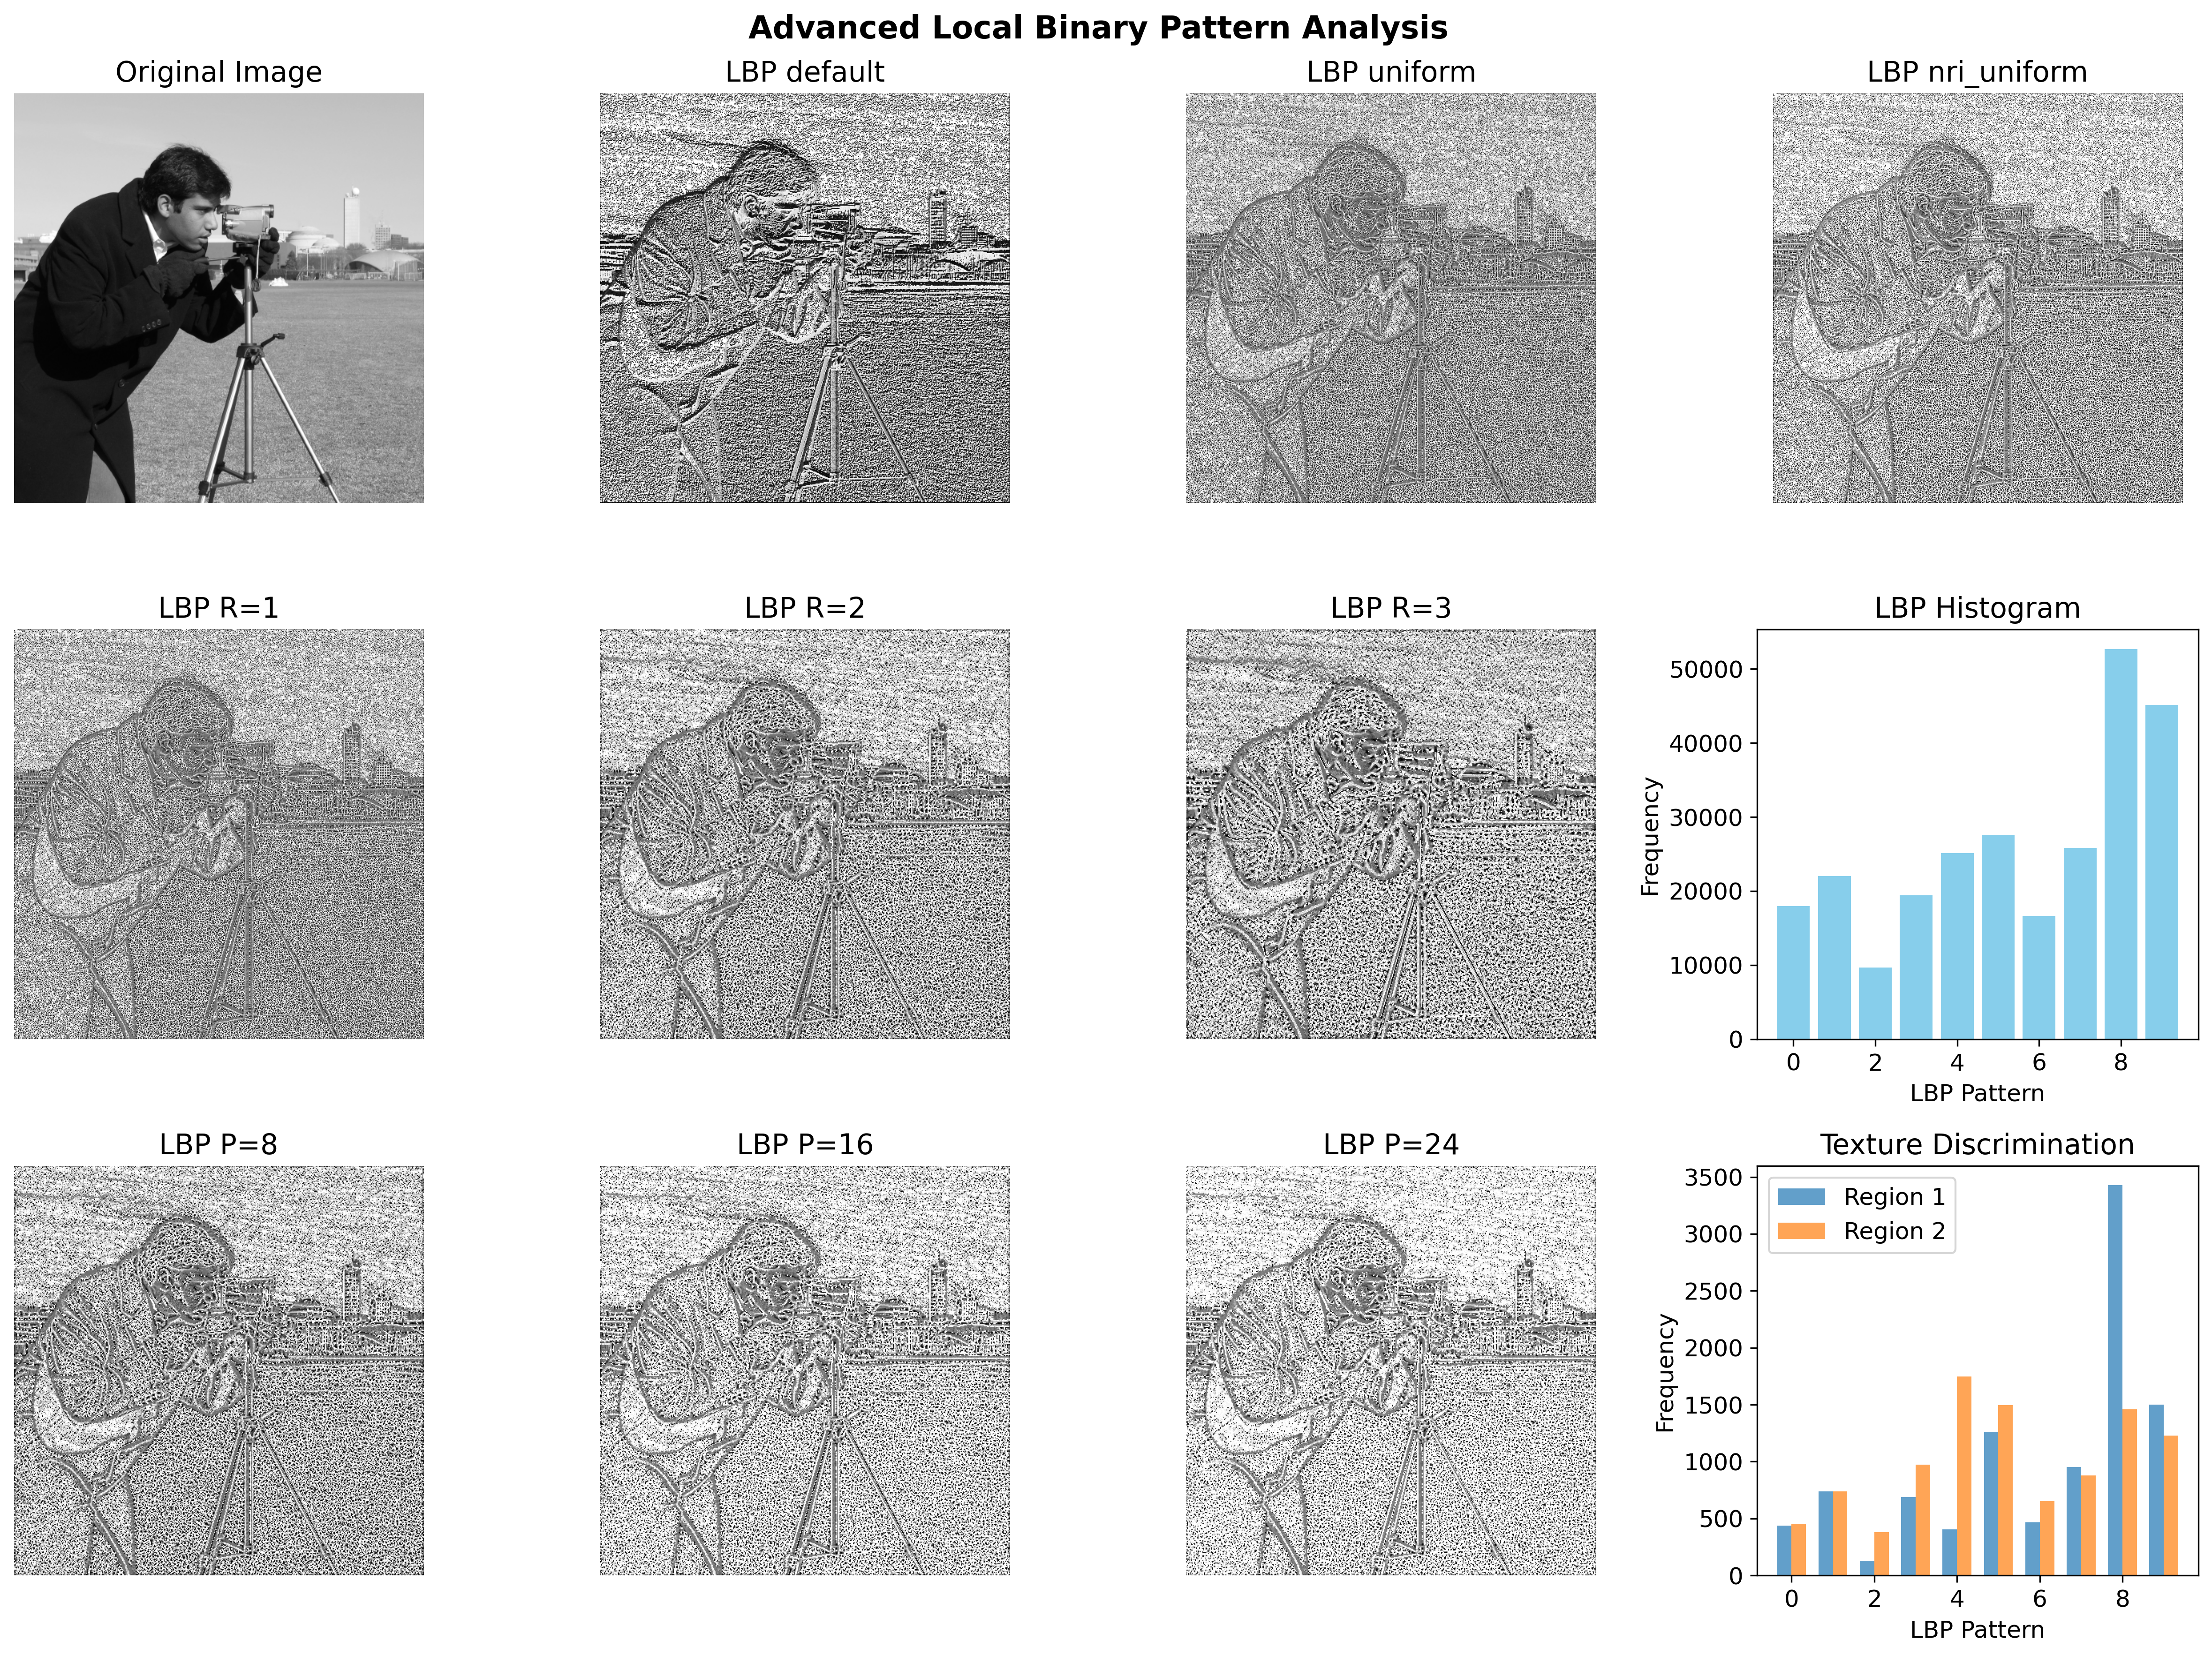
\includegraphics[width=0.8\textwidth,height=0.65\textheight,keepaspectratio]{../figures/advanced_lbp.png}
    \end{center}
\end{frame}

\begin{frame}{LBP Applications and Variants}
    \begin{columns}[c]
        \begin{column}{0.5\textwidth}
            \textbf{LBP Variants:}
            \begin{itemize}
                \item Uniform patterns
                \item Rotation invariant
                \item Multi-scale analysis
                \item Variance measures
            \end{itemize}
        \end{column}
        \begin{column}{0.5\textwidth}
            \textbf{Applications:}
            \begin{itemize}
                \item Face recognition
                \item Texture classification
                \item Surface inspection
                \item Medical imaging
            \end{itemize}
        \end{column}
    \end{columns}
\end{frame}

\begin{frame}{Gabor Filters for Texture}
    \textbf{2D Gabor Function:}
    \begin{align}
        g(x,y) &= \frac{1}{2\pi\sigma_x\sigma_y} \exp\left(-\frac{1}{2}\left[\frac{x'^2}{\sigma_x^2} + \frac{y'^2}{\sigma_y^2}\right]\right) \cos(2\pi fx' + \phi)
    \end{align}

    Where:
    \begin{align}
        x' &= x\cos\theta + y\sin\theta \\
        y' &= -x\sin\theta + y\cos\theta
    \end{align}

    \textbf{Parameters:}
    \begin{itemize}
        \item $\sigma_x, \sigma_y$: Standard deviations (scale)
        \item $f$: Frequency of the sinusoidal wave
        \item $\theta$: Orientation of the filter
        \item $\phi$: Phase offset
    \end{itemize}
\end{frame}

% Corner Detection Section
\section{Corner Detection}

\begin{frame}{Corner Detection: Harris Detector}
    \begin{center}
        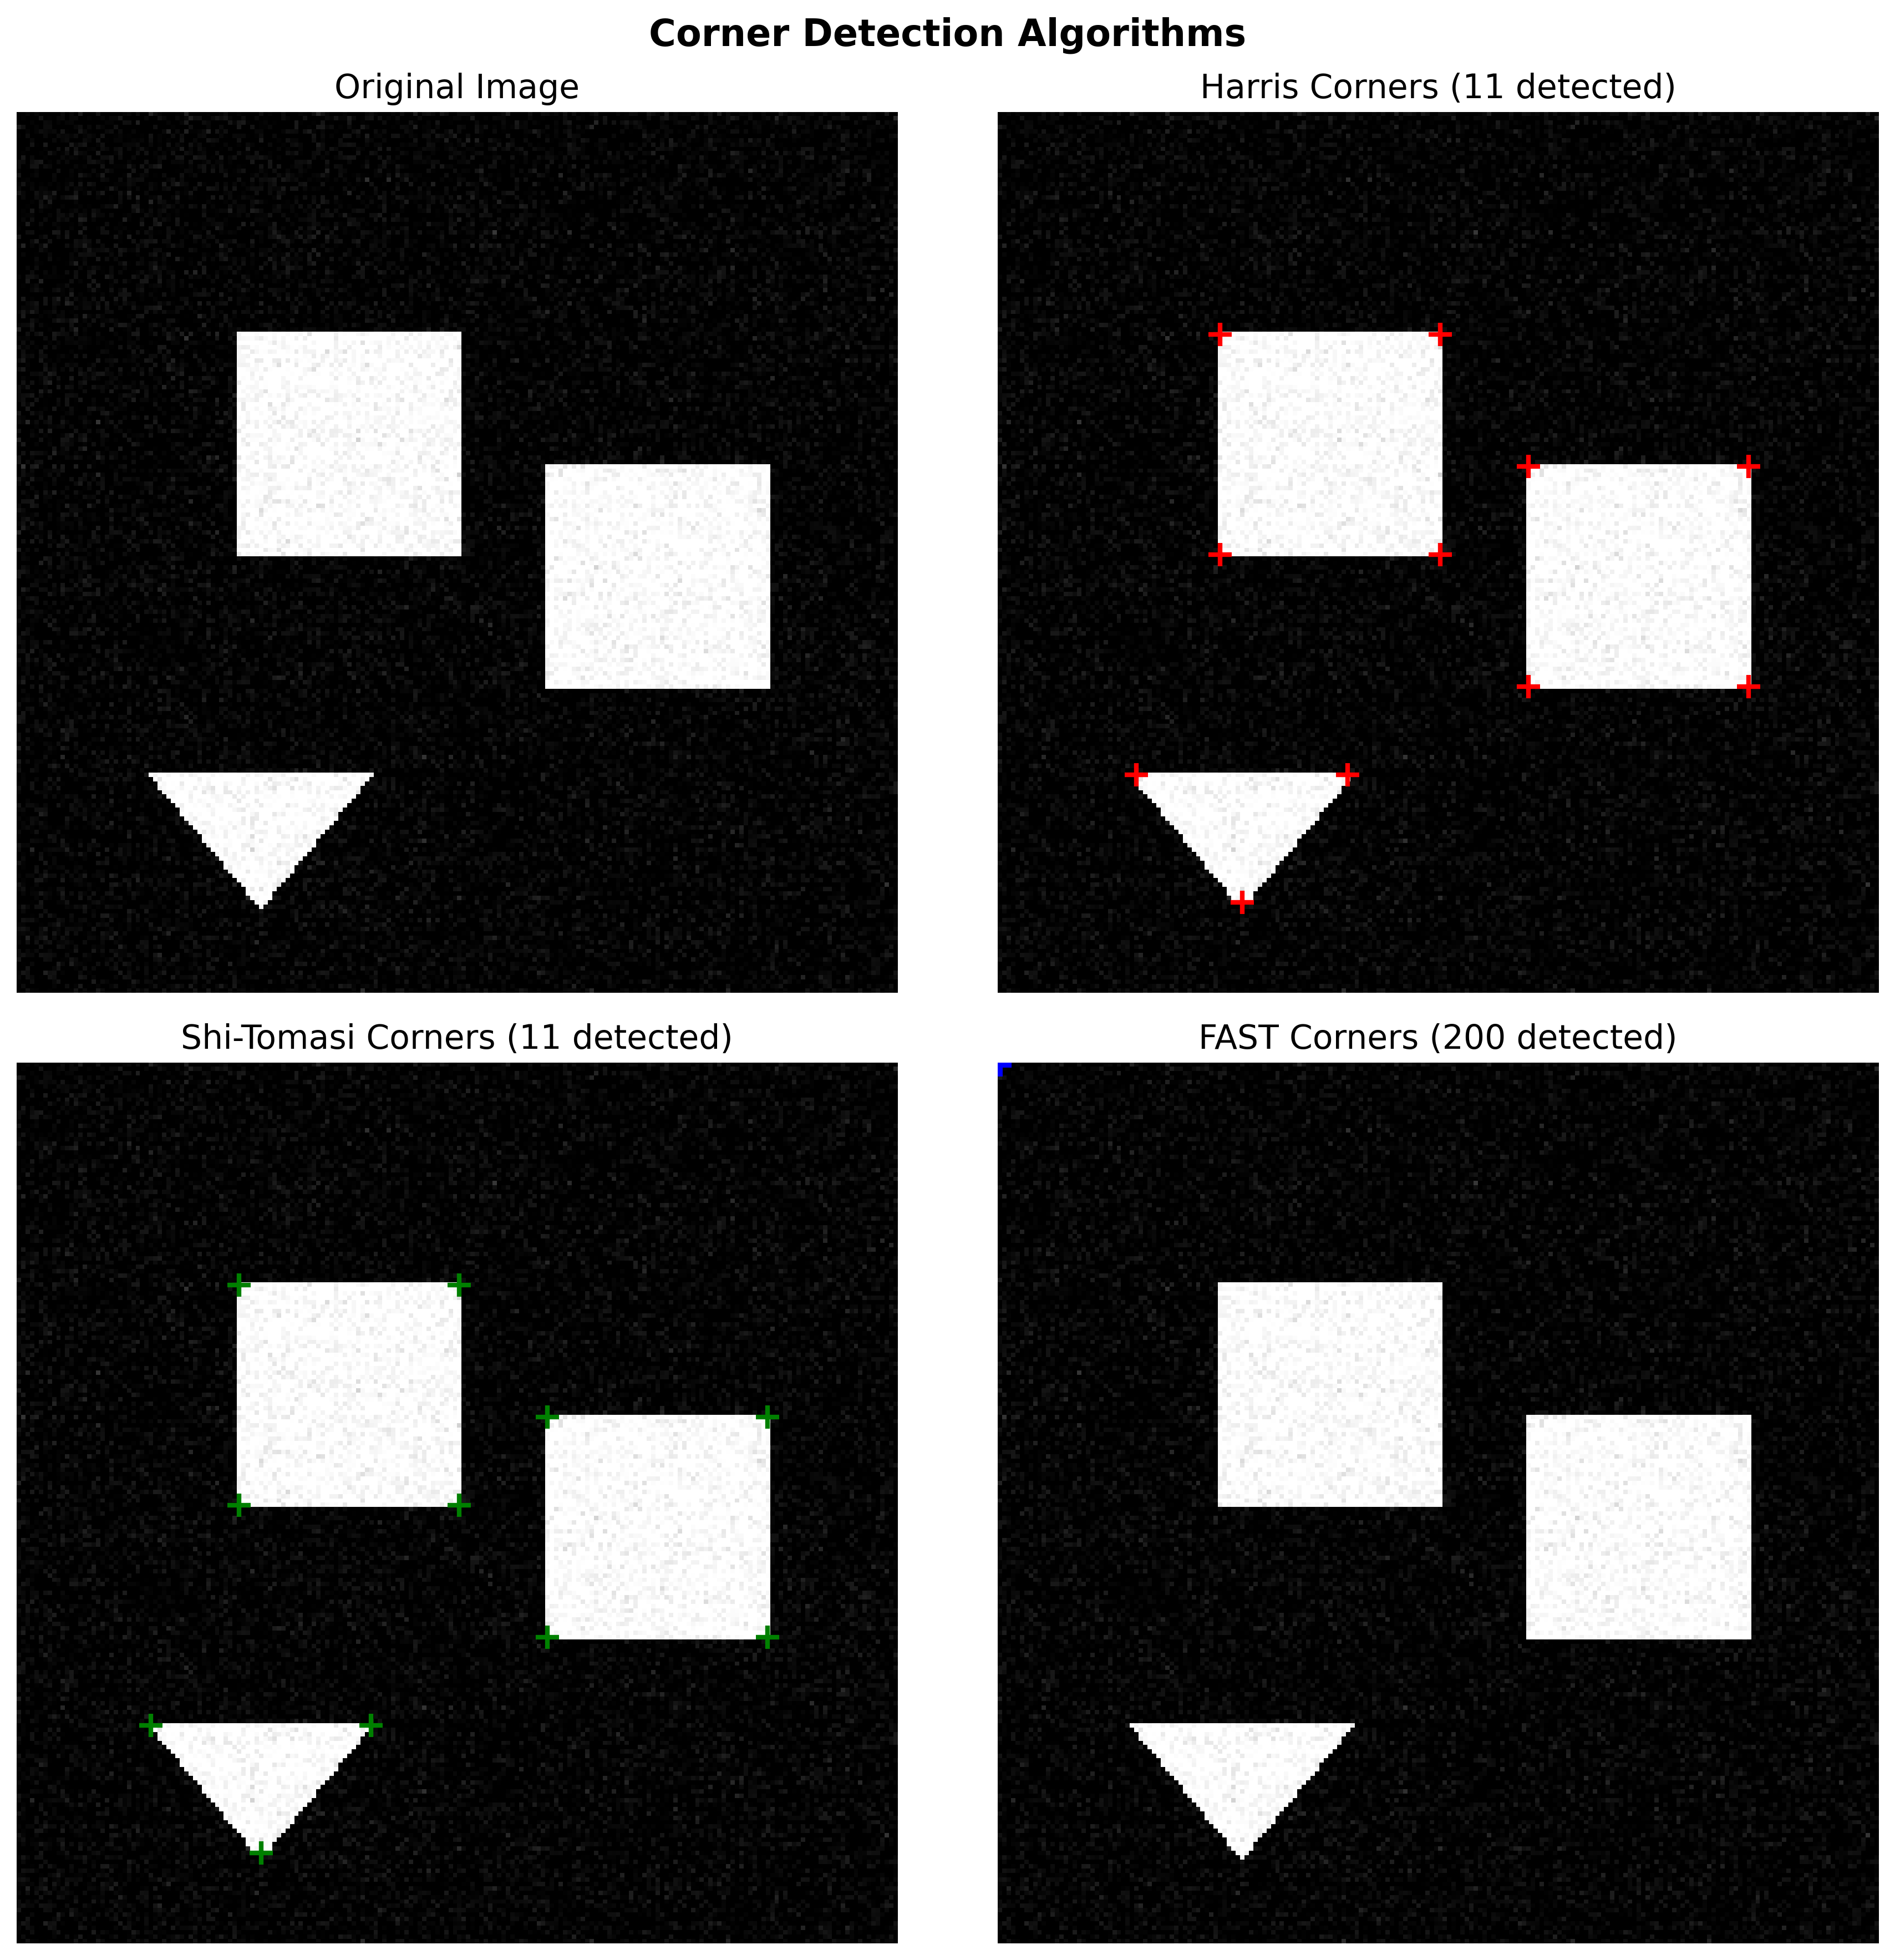
\includegraphics[width=0.65\textwidth,height=0.55\textheight,keepaspectratio]{../figures/corner_detection.png}
    \end{center}

    \textbf{Harris Corner Response:}
    \begin{align}
        R &= \det(M) - k \cdot \text{trace}(M)^2 \\
        M &= \begin{bmatrix}
            \sum I_x^2 & \sum I_x I_y \\
            \sum I_x I_y & \sum I_y^2
        \end{bmatrix}
    \end{align}

    Where $k$ is an empirical constant (typically $k = 0.04$).
\end{frame}

\begin{frame}{Corner Detection Methods}
    \begin{columns}[c]
        \begin{column}{0.5\textwidth}
            \textbf{Harris Corner Detector:}
            \begin{itemize}
                \item Based on autocorrelation
                \item Scale dependent
                \item Good repeatability
                \item Rotation invariant
            \end{itemize}

            \textbf{Shi-Tomasi Method:}
            \begin{itemize}
                \item Uses minimum eigenvalue
                \item Better corner selection
                \item More stable features
            \end{itemize}
        \end{column}
        \begin{column}{0.5\textwidth}
            \textbf{FAST Detector:}
            \begin{itemize}
                \item Computationally efficient
                \item Real-time applications
                \item Machine learning optimized
                \item Good performance
            \end{itemize}

            \textbf{Applications:}
            \begin{itemize}
                \item Object tracking
                \item Image registration
                \item 3D reconstruction
                \item SLAM systems
            \end{itemize}
        \end{column}
    \end{columns}
\end{frame}

% Advanced Feature Descriptors Section
\section{Advanced Feature Descriptors}

\begin{frame}{SIFT Features}
    \begin{center}
        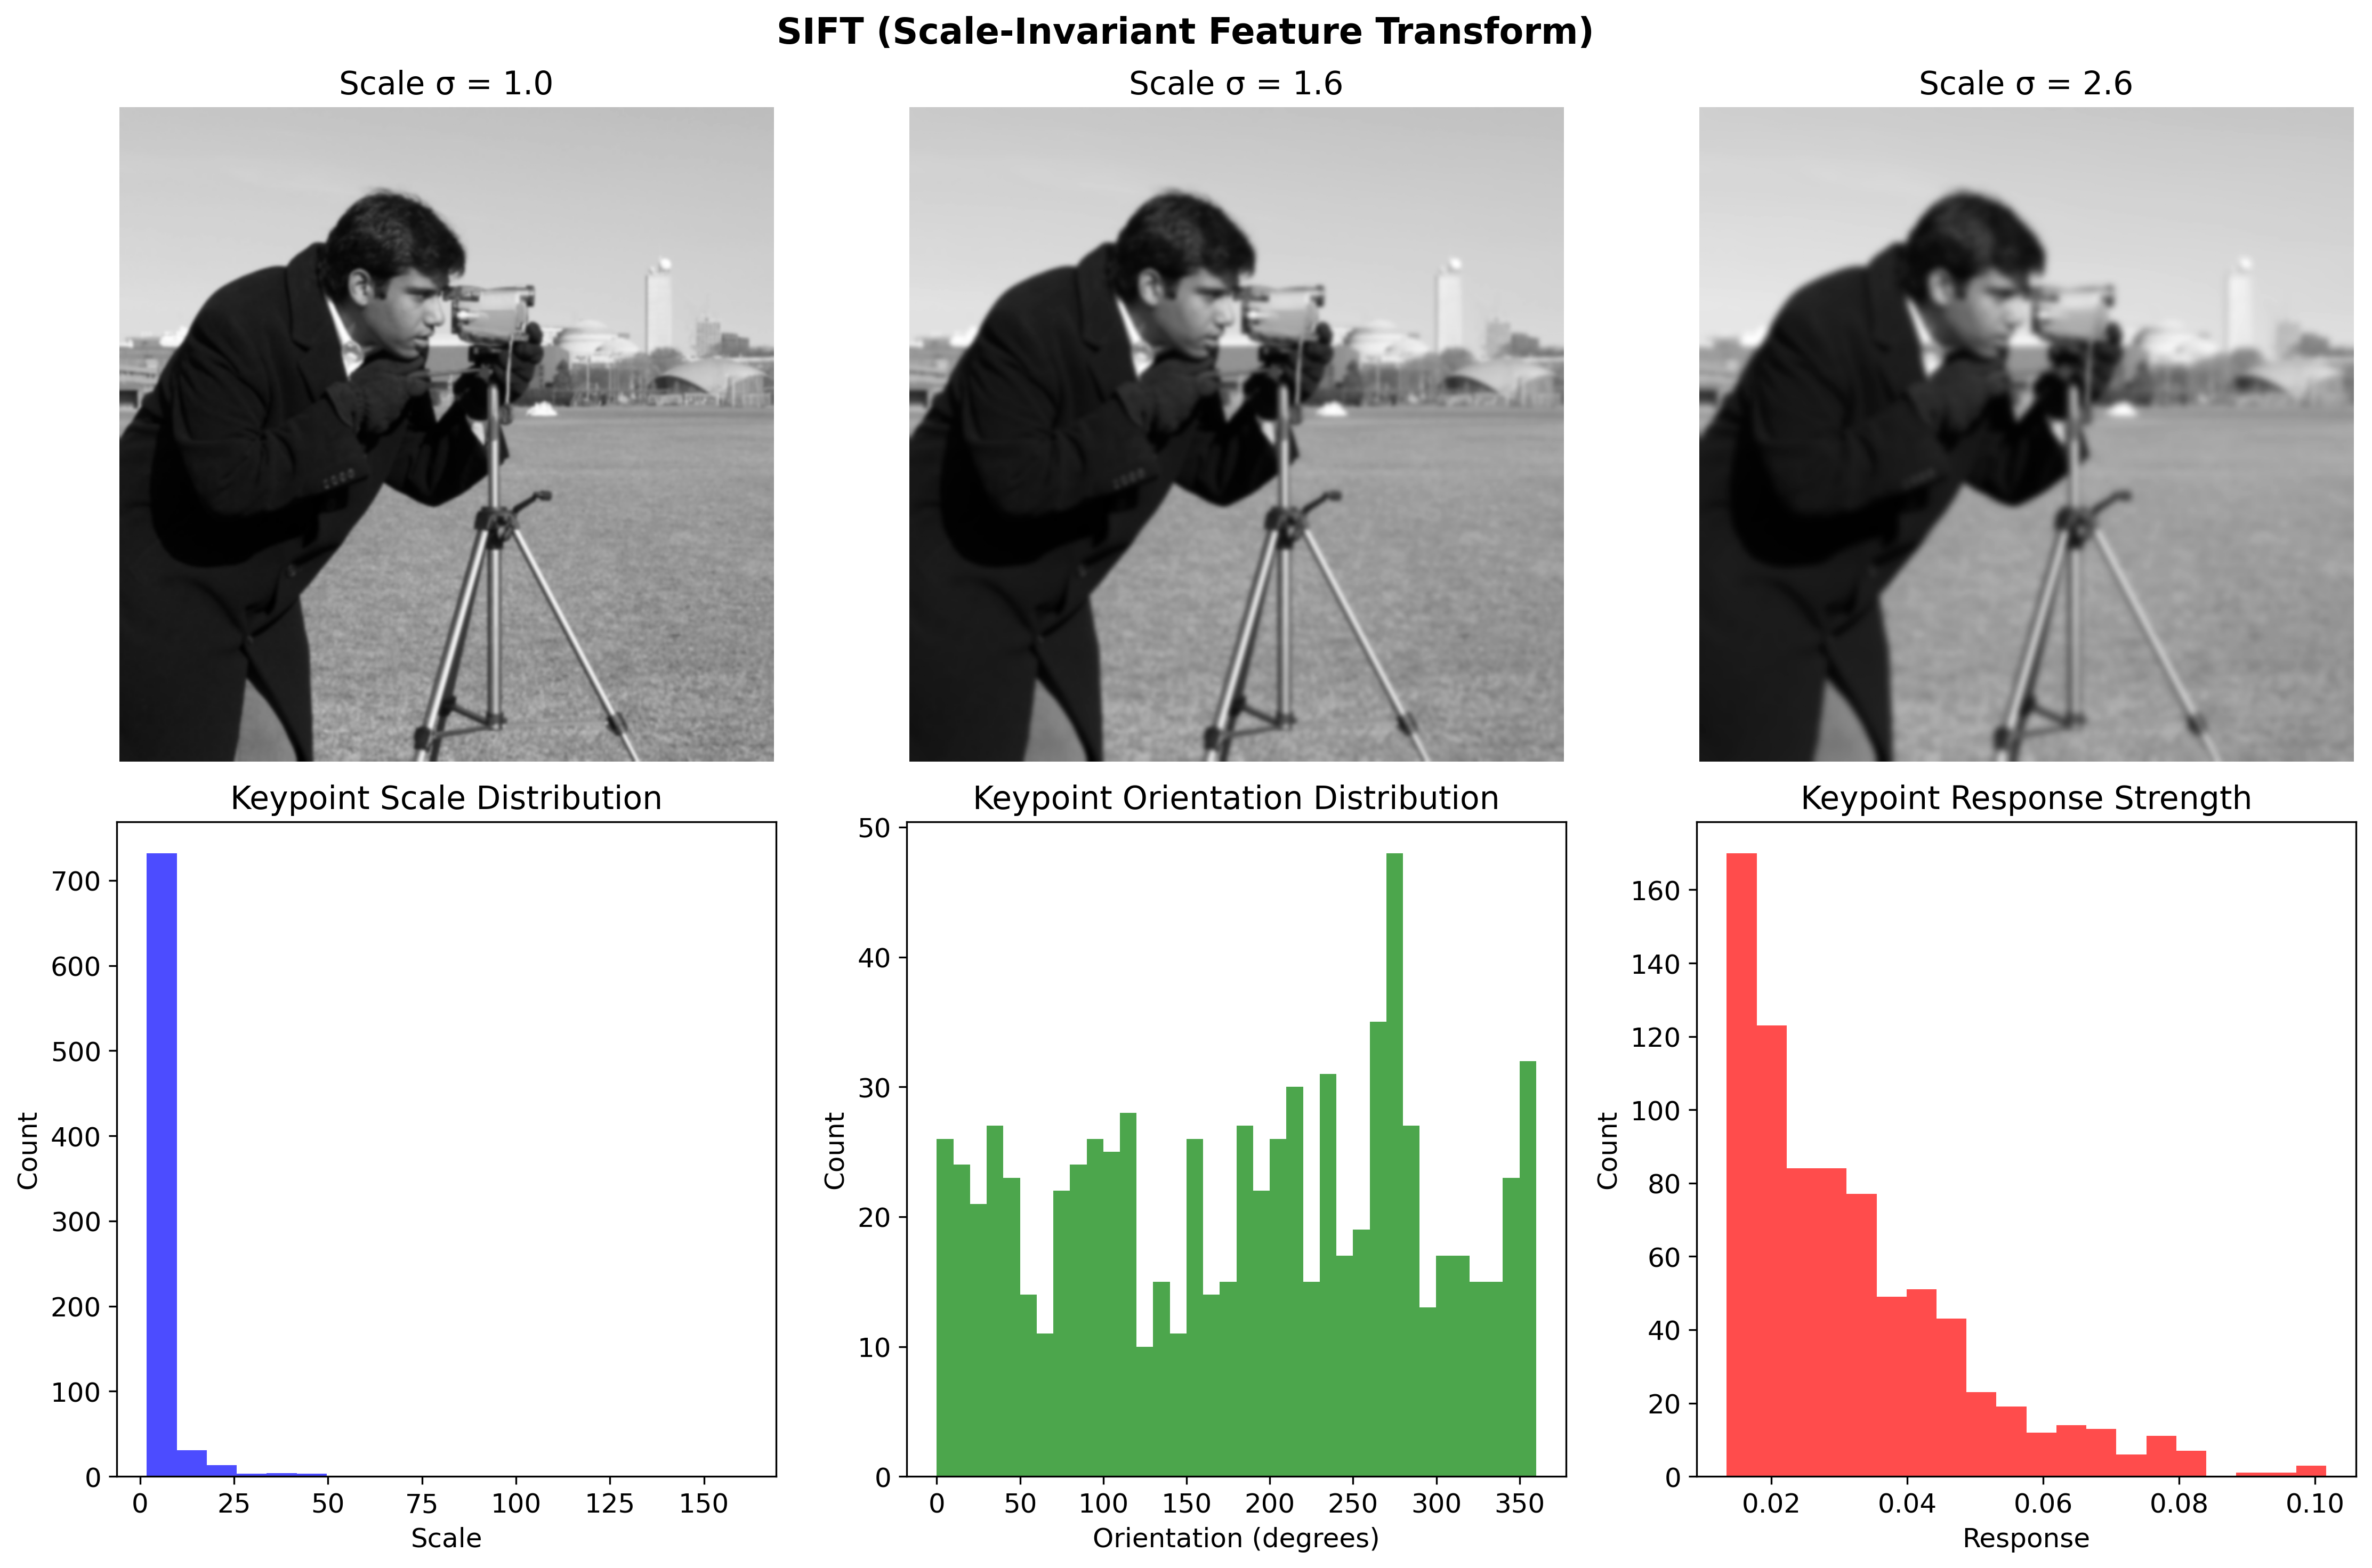
\includegraphics[width=0.8\textwidth,height=0.6\textheight,keepaspectratio]{../figures/sift_features.png}
    \end{center}

    \begin{alertblock}{SIFT Properties}
        \textbf{Scale-Invariant Feature Transform} provides features that are invariant to:
        scale, rotation, illumination changes, and partially invariant to affine transformations.
    \end{alertblock}
\end{frame}

\begin{frame}{SIFT Algorithm Overview}
    \textbf{Four Main Steps:}
    \begin{enumerate}
        \item \textbf{Scale-space extrema detection}
        \begin{itemize}
            \item Use Difference of Gaussians (DoG)
            \item Find keypoints across scales
        \end{itemize}

        \item \textbf{Keypoint localization}
        \begin{itemize}
            \item Eliminate low contrast points
            \item Remove edge responses
        \end{itemize}

        \item \textbf{Orientation assignment}
        \begin{itemize}
            \item Compute gradient histograms
            \item Assign dominant orientations
        \end{itemize}

        \item \textbf{Descriptor generation}
        \begin{itemize}
            \item 16×16 neighborhood around keypoint
            \item 4×4 sub-regions with 8-bin histograms
            \item 128-dimensional feature vector
        \end{itemize}
    \end{enumerate}
\end{frame}

\begin{frame}{ORB Features}
    \begin{center}
        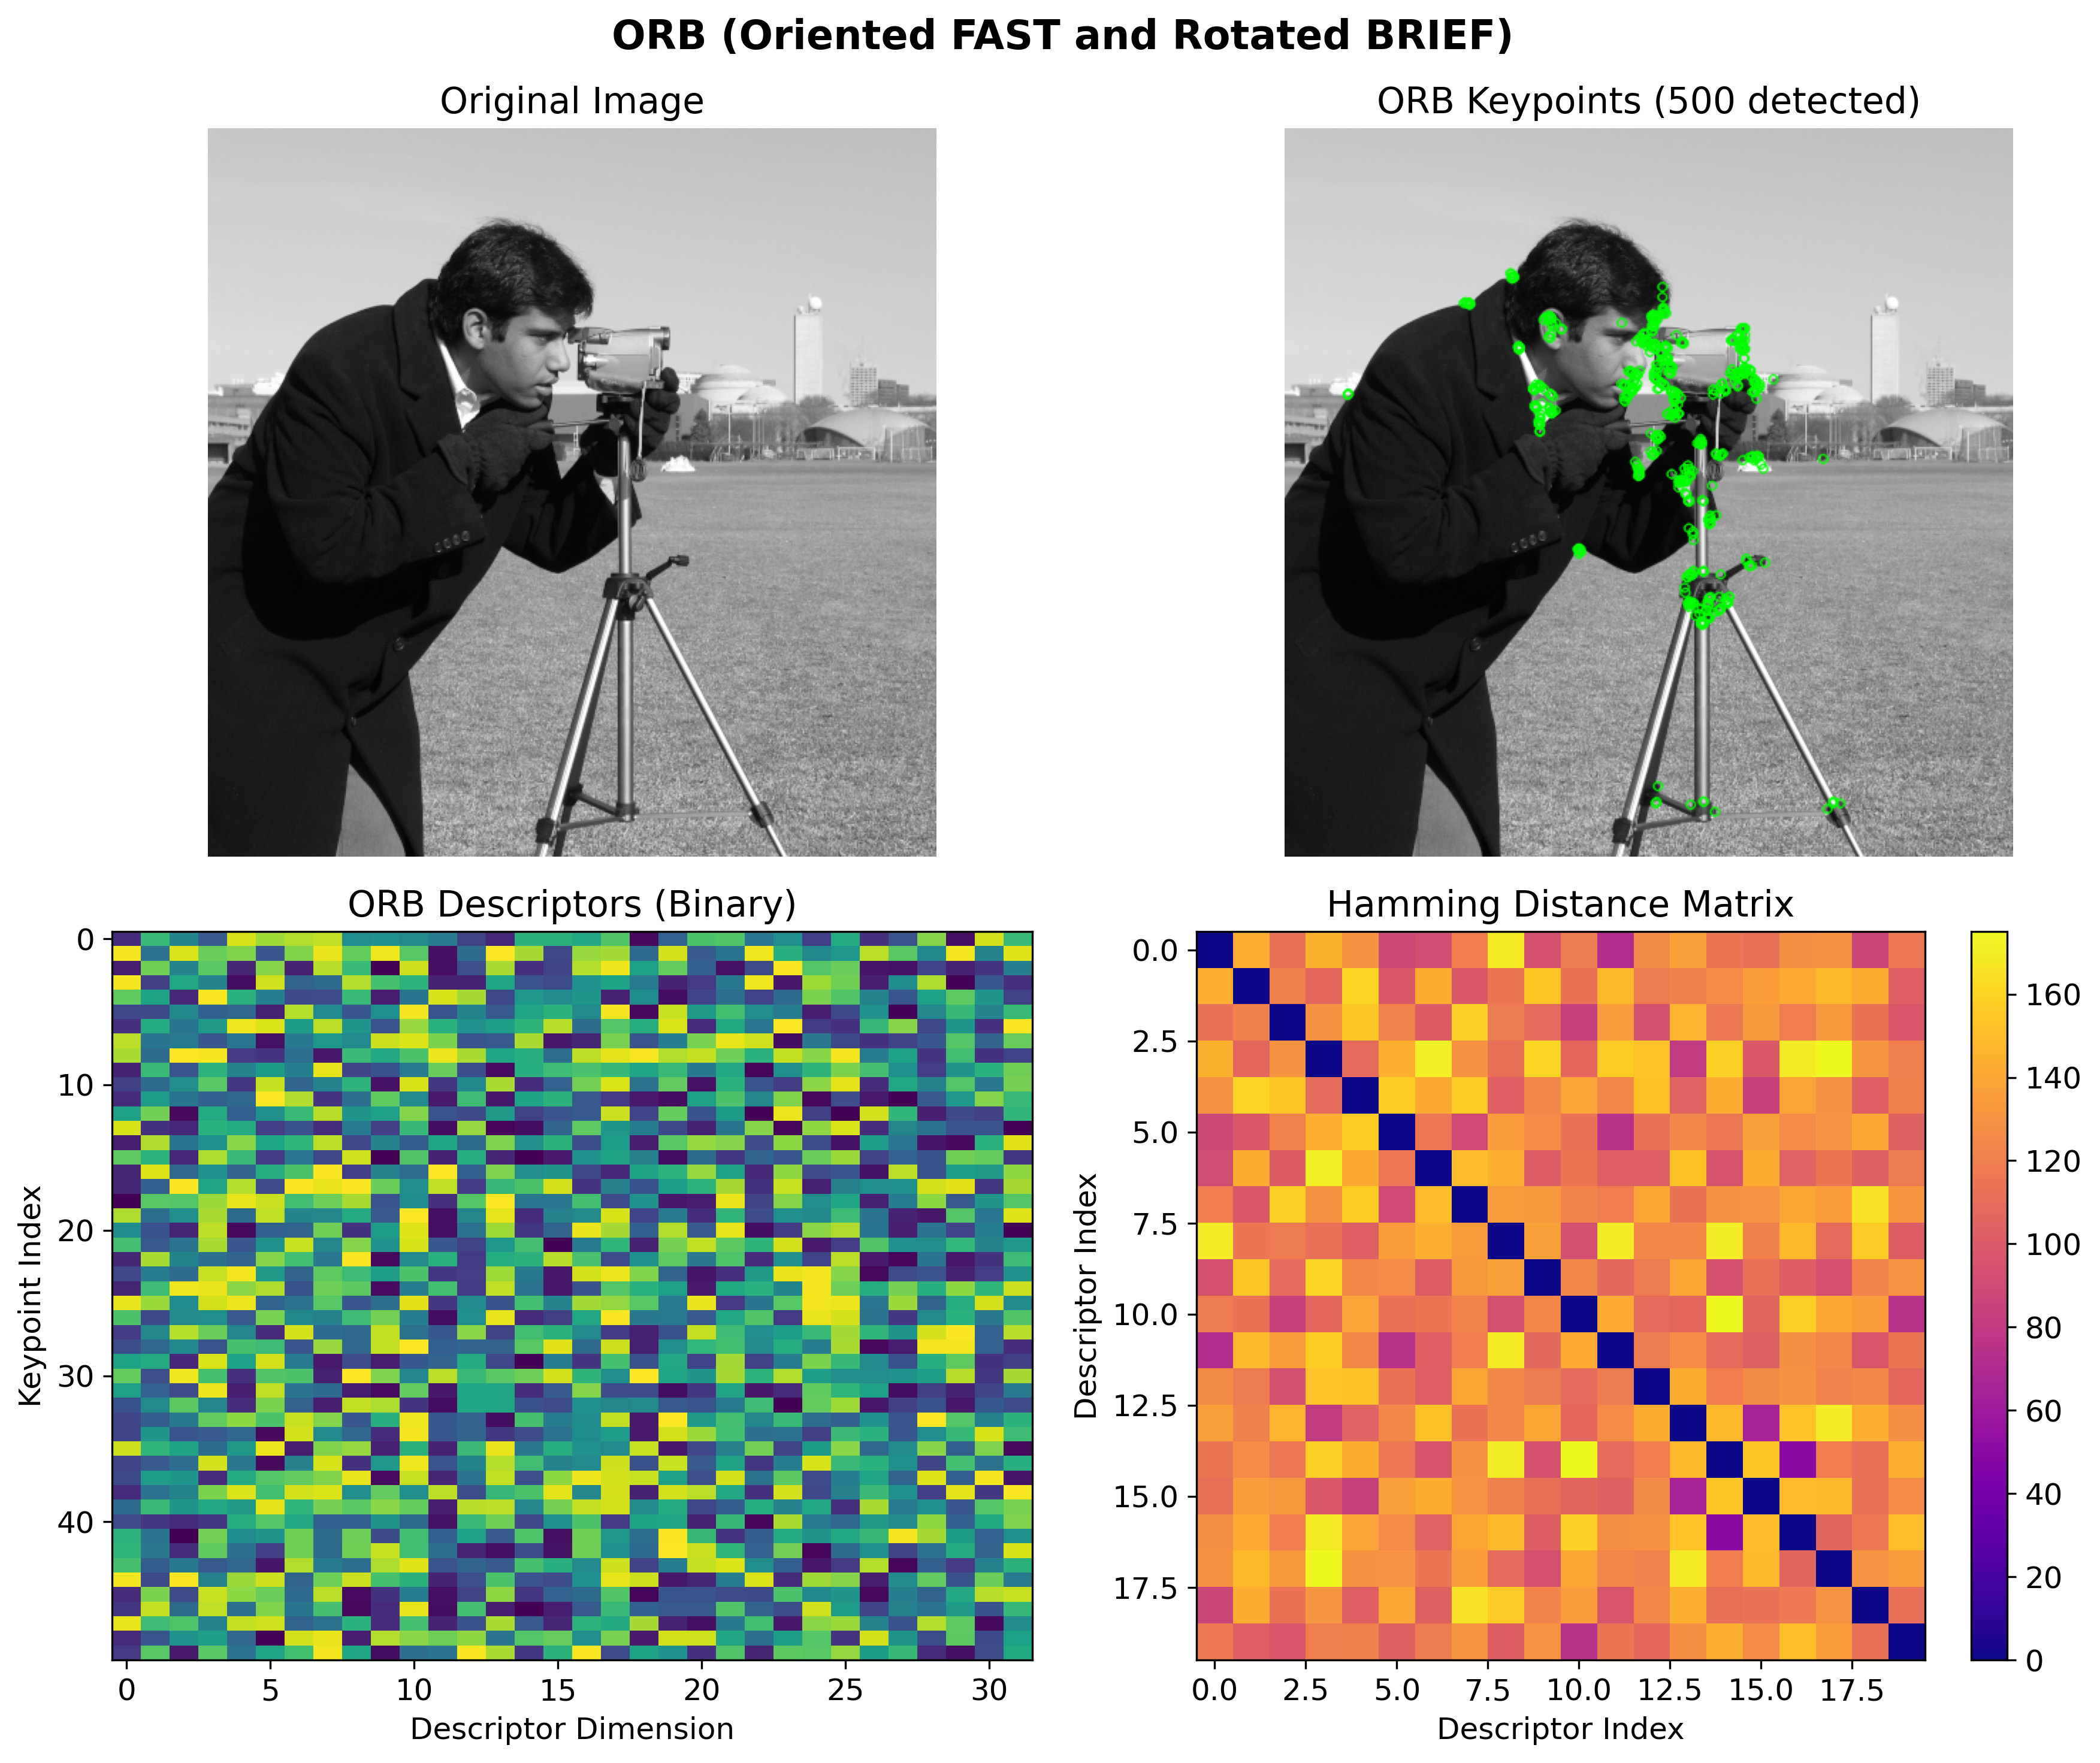
\includegraphics[width=0.75\textwidth,height=0.55\textheight,keepaspectratio]{../figures/orb_features.png}
    \end{center}

    \begin{columns}[c]
        \begin{column}{0.5\textwidth}
            \textbf{ORB = oFAST + rBRIEF}
            \begin{itemize}
                \item Oriented FAST keypoints
                \item Rotated BRIEF descriptors
                \item Binary descriptors
                \item Fast computation
            \end{itemize}
        \end{column}
        \begin{column}{0.5\textwidth}
            \textbf{Advantages:}
            \begin{itemize}
                \item Real-time performance
                \item Low memory usage
                \item Free alternative to SIFT
                \item Good matching performance
            \end{itemize}
        \end{column}
    \end{columns}
\end{frame}

\begin{frame}{HOG Features}
    \begin{center}
        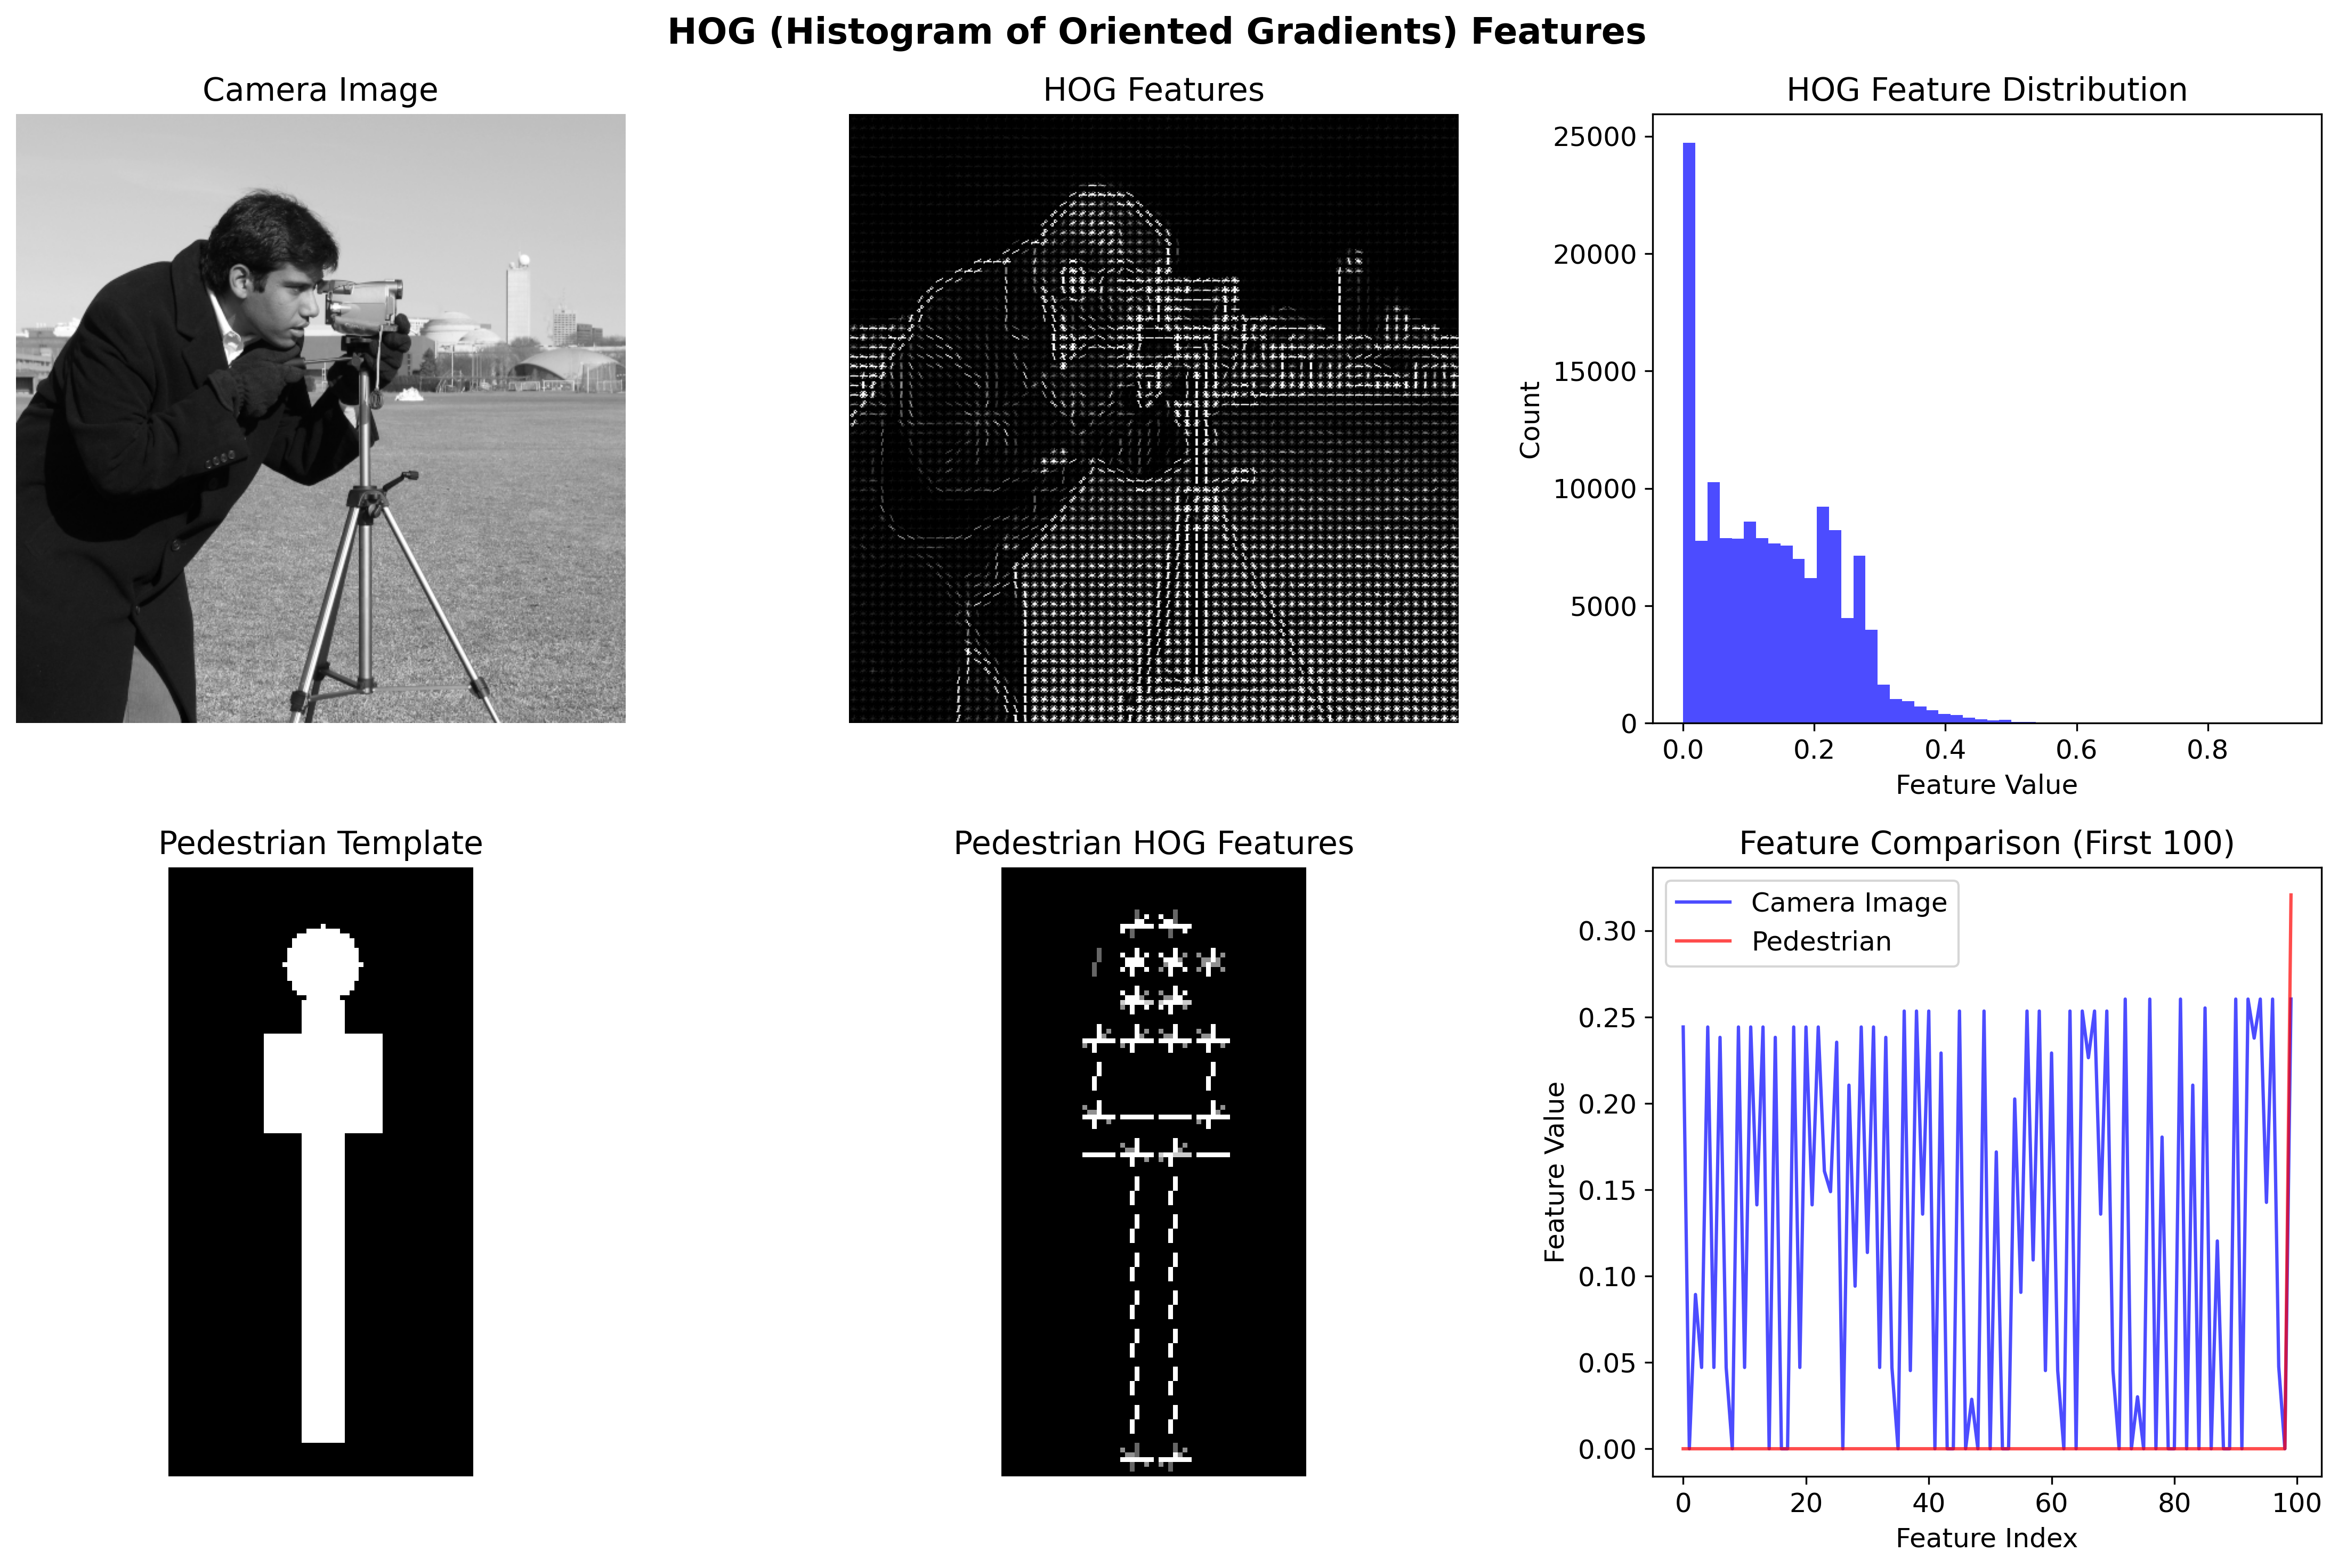
\includegraphics[width=0.8\textwidth,height=0.55\textheight,keepaspectratio]{../figures/hog_features.png}
    \end{center}

    \textbf{Histogram of Oriented Gradients:}
    \begin{itemize}
        \item Divide image into cells (e.g., 8×8 pixels)
        \item Compute gradient orientation histogram for each cell
        \item Normalize over larger blocks (e.g., 2×2 cells)
        \item Concatenate histograms to form feature vector
    \end{itemize}
\end{frame}

\begin{frame}{Feature Matching}
    \begin{center}
        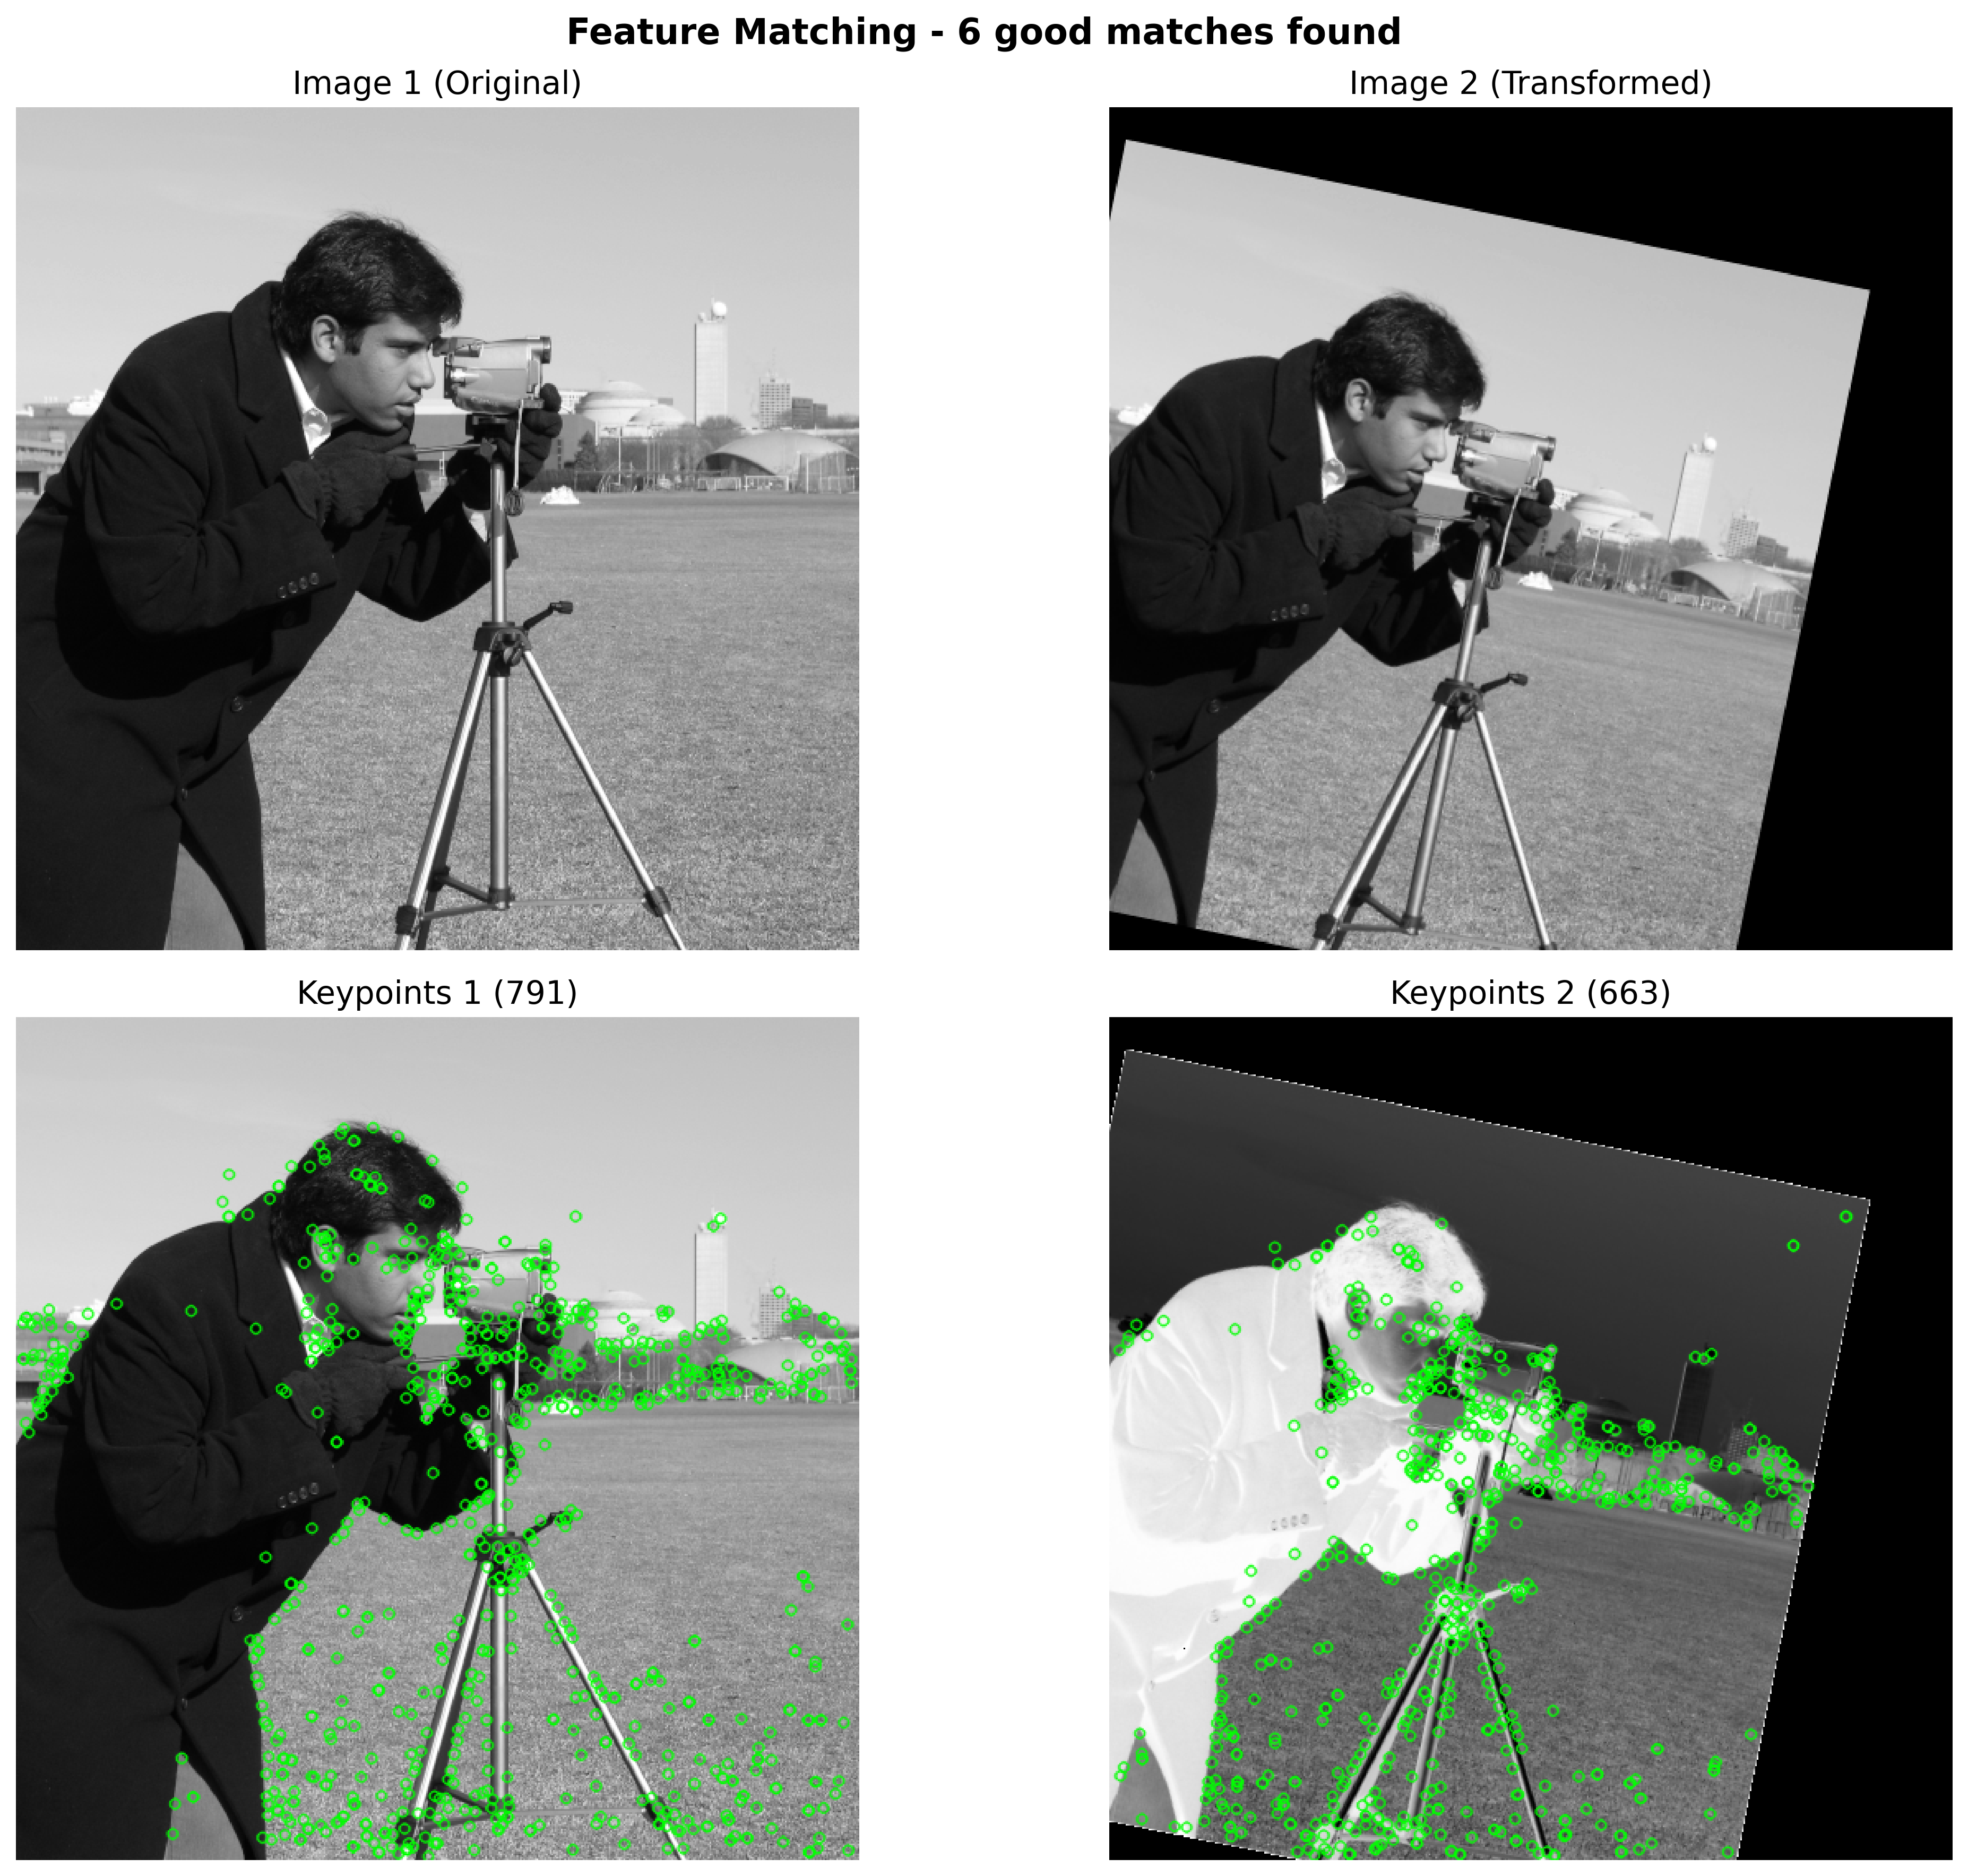
\includegraphics[width=0.75\textwidth,height=0.55\textheight,keepaspectratio]{../figures/feature_matching.png}
    \end{center}

    \textbf{Matching Strategies:}
    \begin{itemize}
        \item \textbf{Brute Force:} Compare all descriptors
        \item \textbf{FLANN:} Fast Library for Approximate Nearest Neighbors
        \item \textbf{Ratio Test:} Lowe's criterion for good matches
        \item \textbf{RANSAC:} Remove outliers for geometric consistency
    \end{itemize}
\end{frame}

\begin{frame}{Feature Matching Lines}
    \begin{center}
        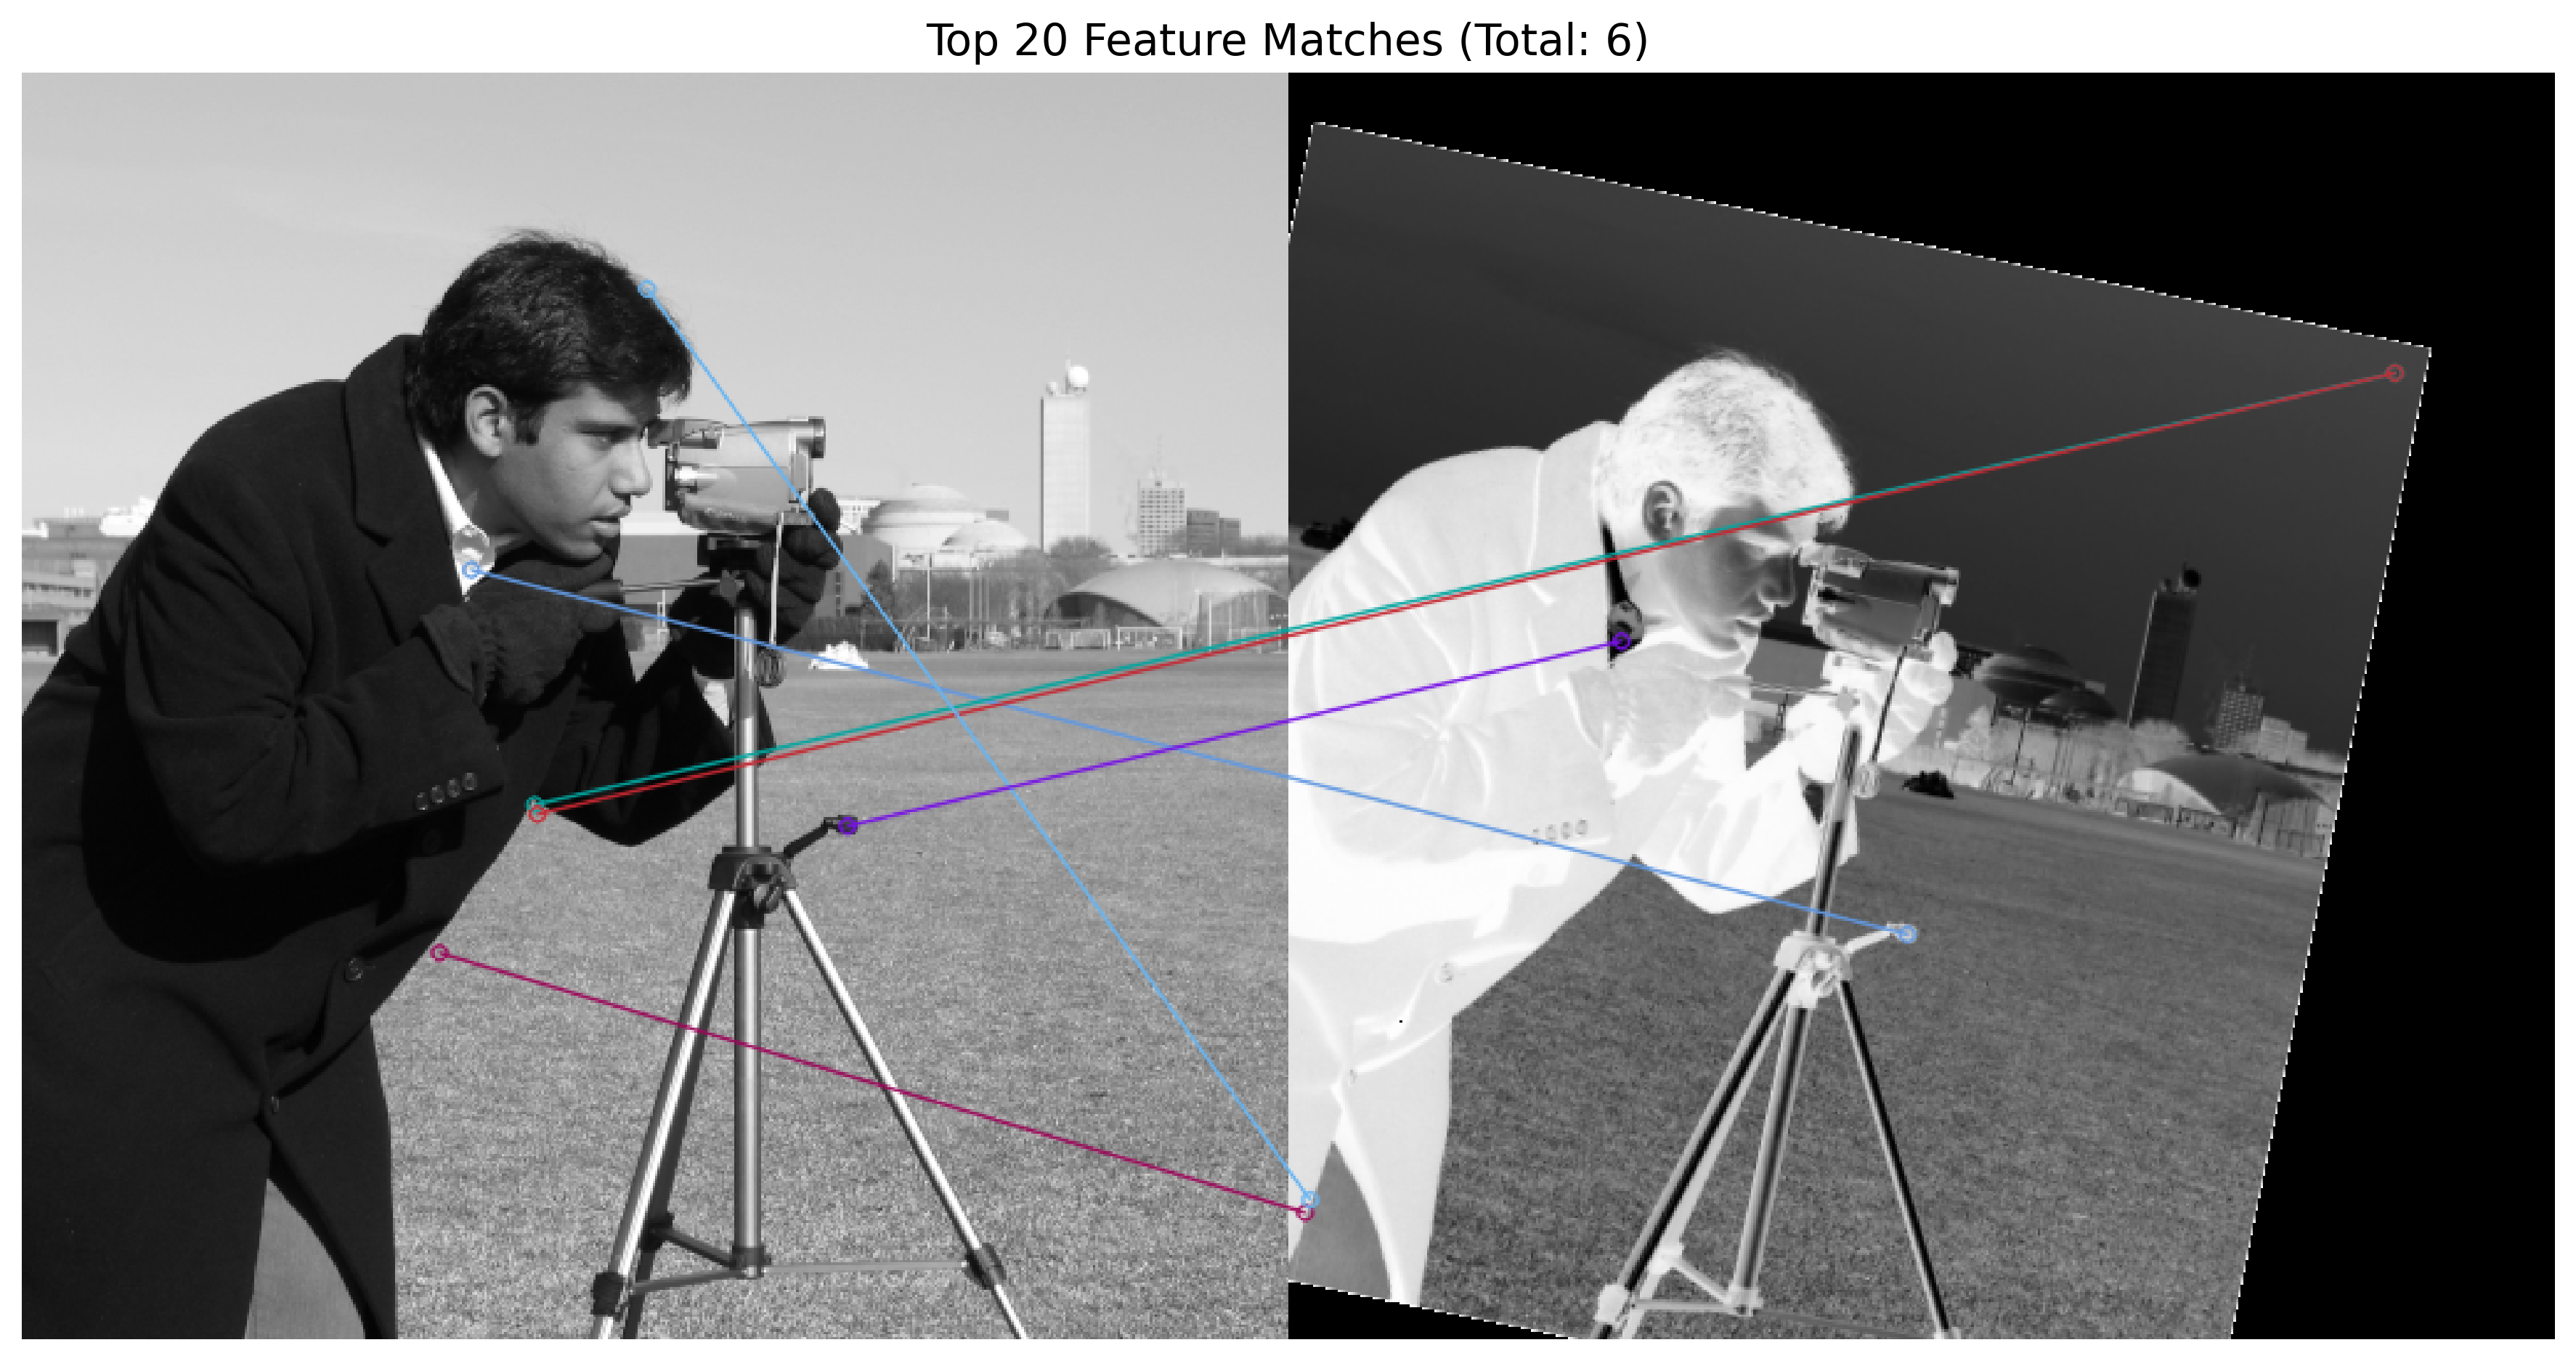
\includegraphics[width=0.85\textwidth,height=0.5\textheight,keepaspectratio]{../figures/feature_matches_lines.png}
    \end{center}

    \begin{alertblock}{Quality Assessment}
        Good matches should be consistent with the underlying geometric transformation between images.
    \end{alertblock}
\end{frame}

% Applications Section
\section{Real-World Applications}

\begin{frame}{Document Analysis}
    \begin{center}
        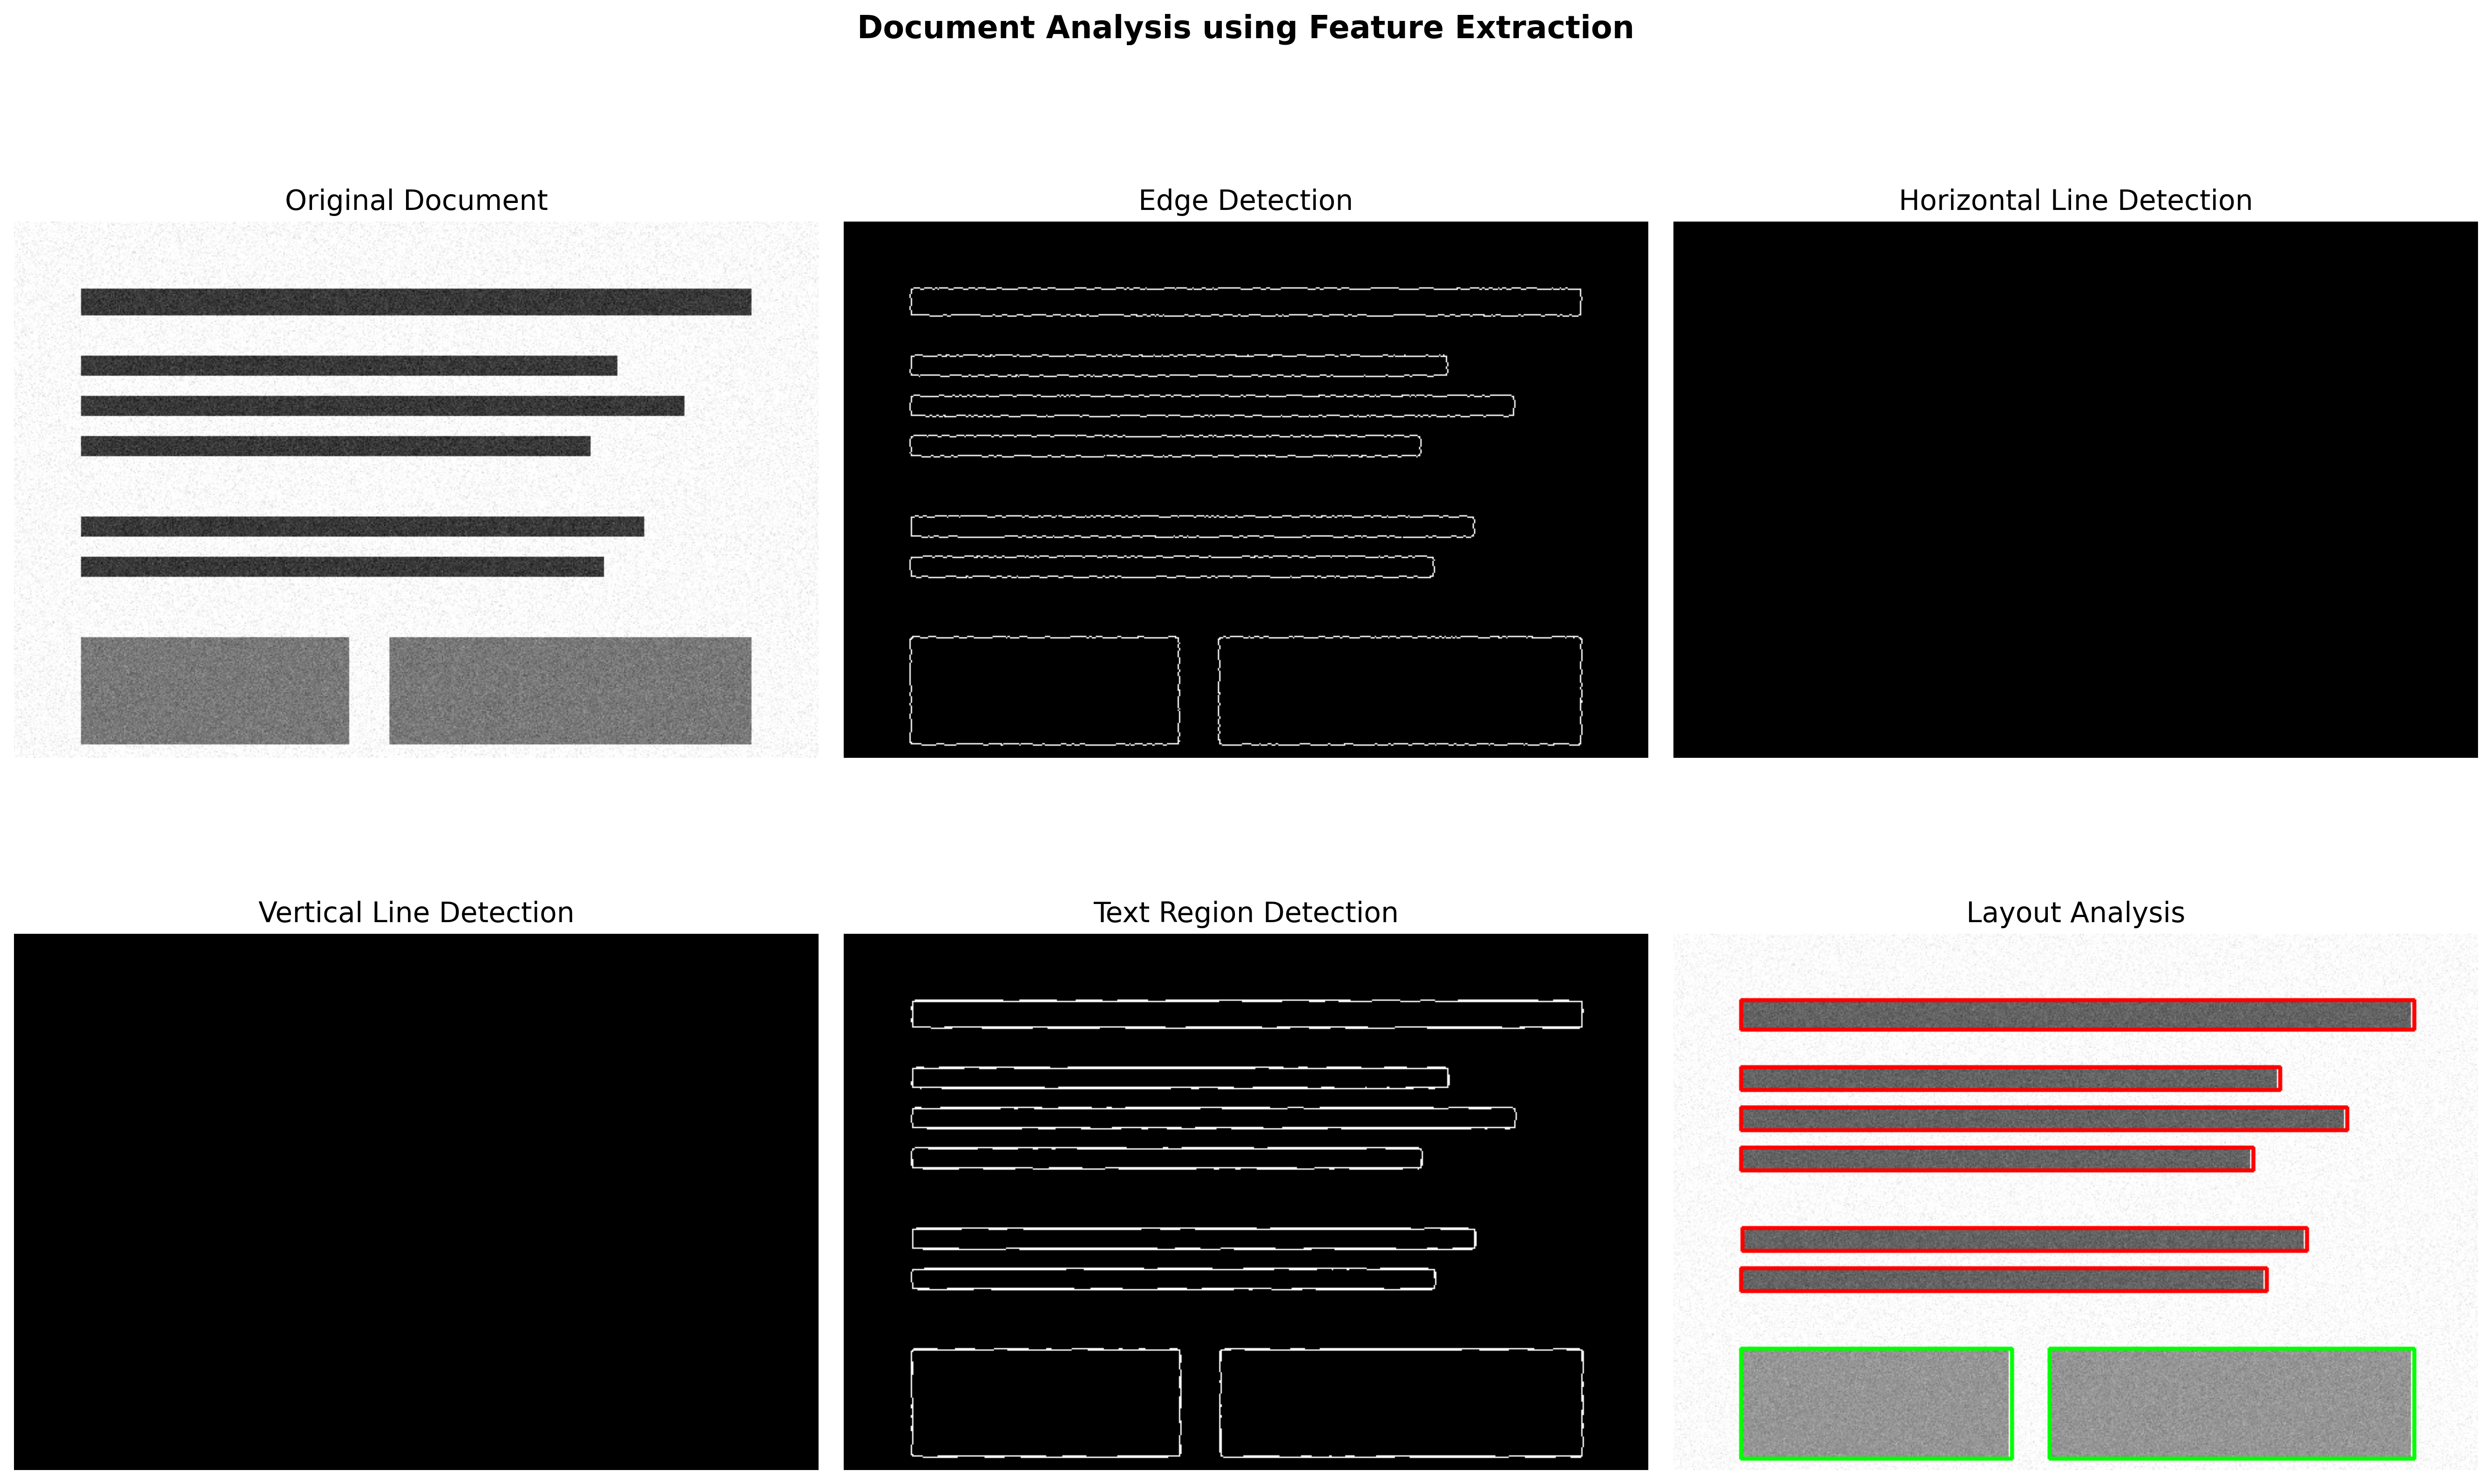
\includegraphics[width=0.75\textwidth,height=0.55\textheight,keepaspectratio]{../figures/document_analysis.png}
    \end{center}

    \textbf{Key Tasks:}
    \begin{itemize}
        \item Text line detection
        \item Layout analysis
        \item Table extraction
        \item Figure identification
    \end{itemize}
\end{frame}

\begin{frame}{Medical Imaging}
    \begin{center}
        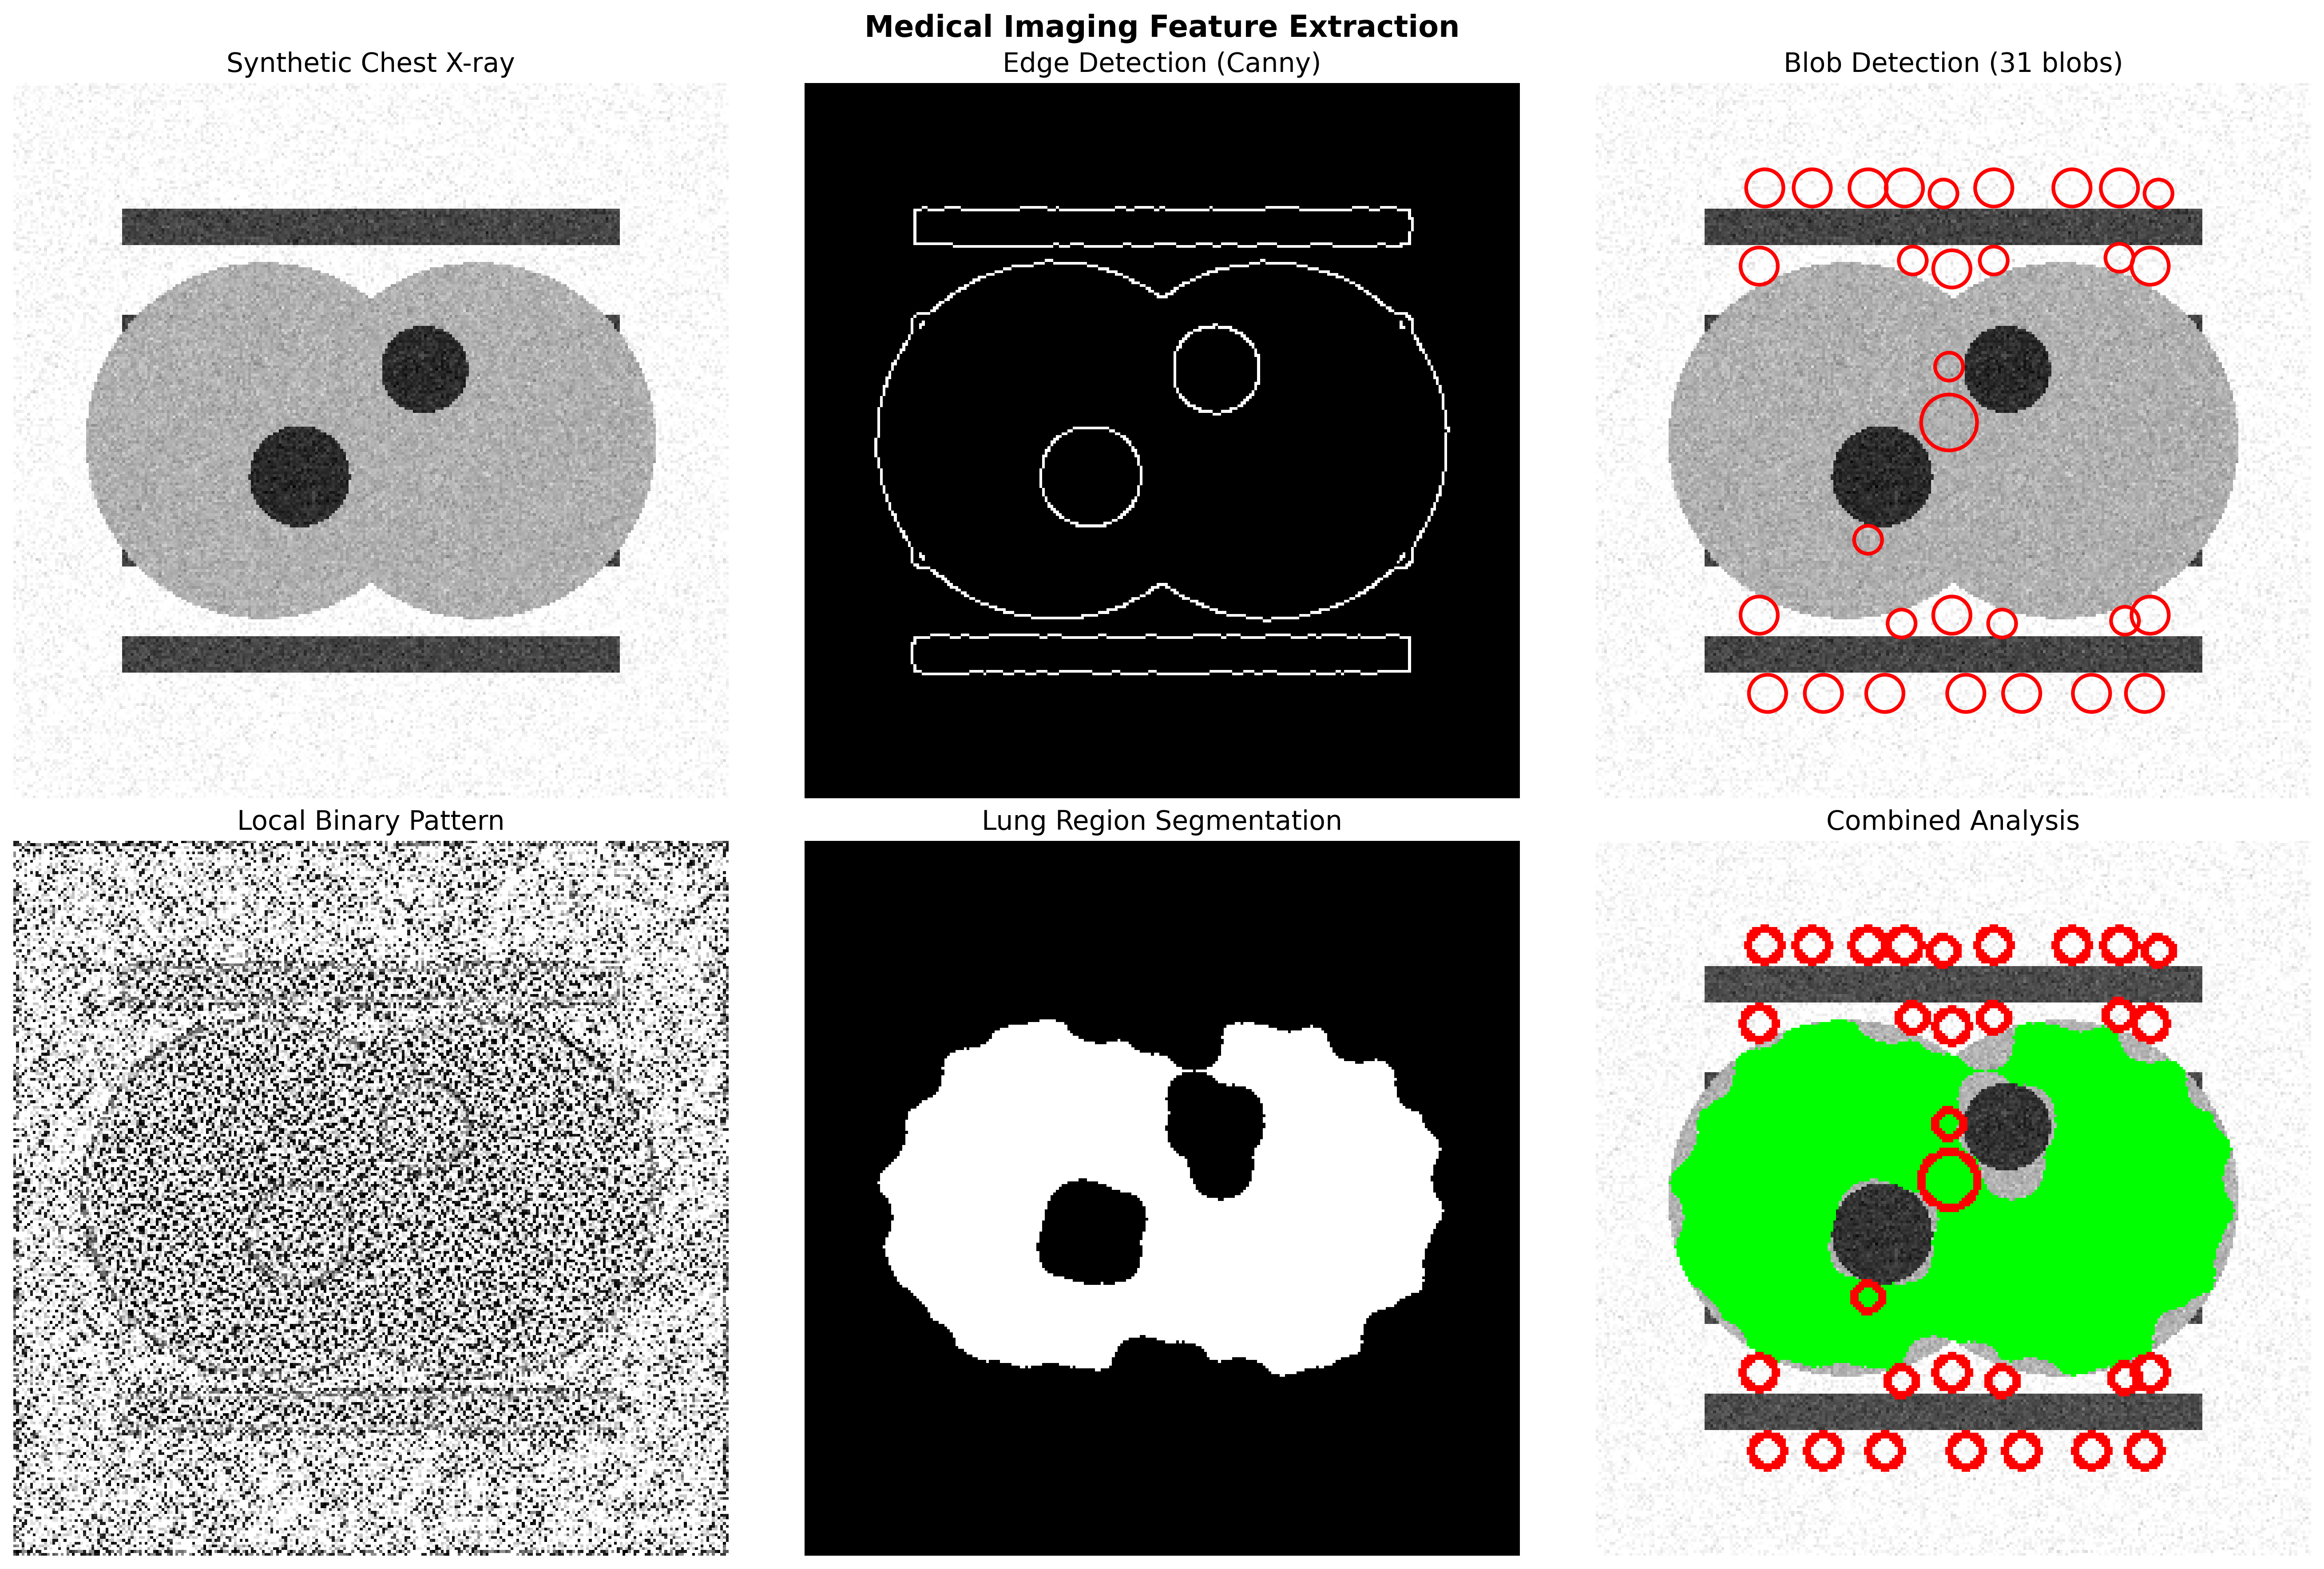
\includegraphics[width=0.75\textwidth,height=0.55\textheight,keepaspectratio]{../figures/medical_imaging.png}
    \end{center}

    \textbf{Applications:}
    \begin{itemize}
        \item Organ segmentation
        \item Abnormality detection
        \item Treatment planning
        \item Diagnostic assistance
    \end{itemize}
\end{frame}

\begin{frame}{Industrial Quality Inspection}
    \begin{center}
        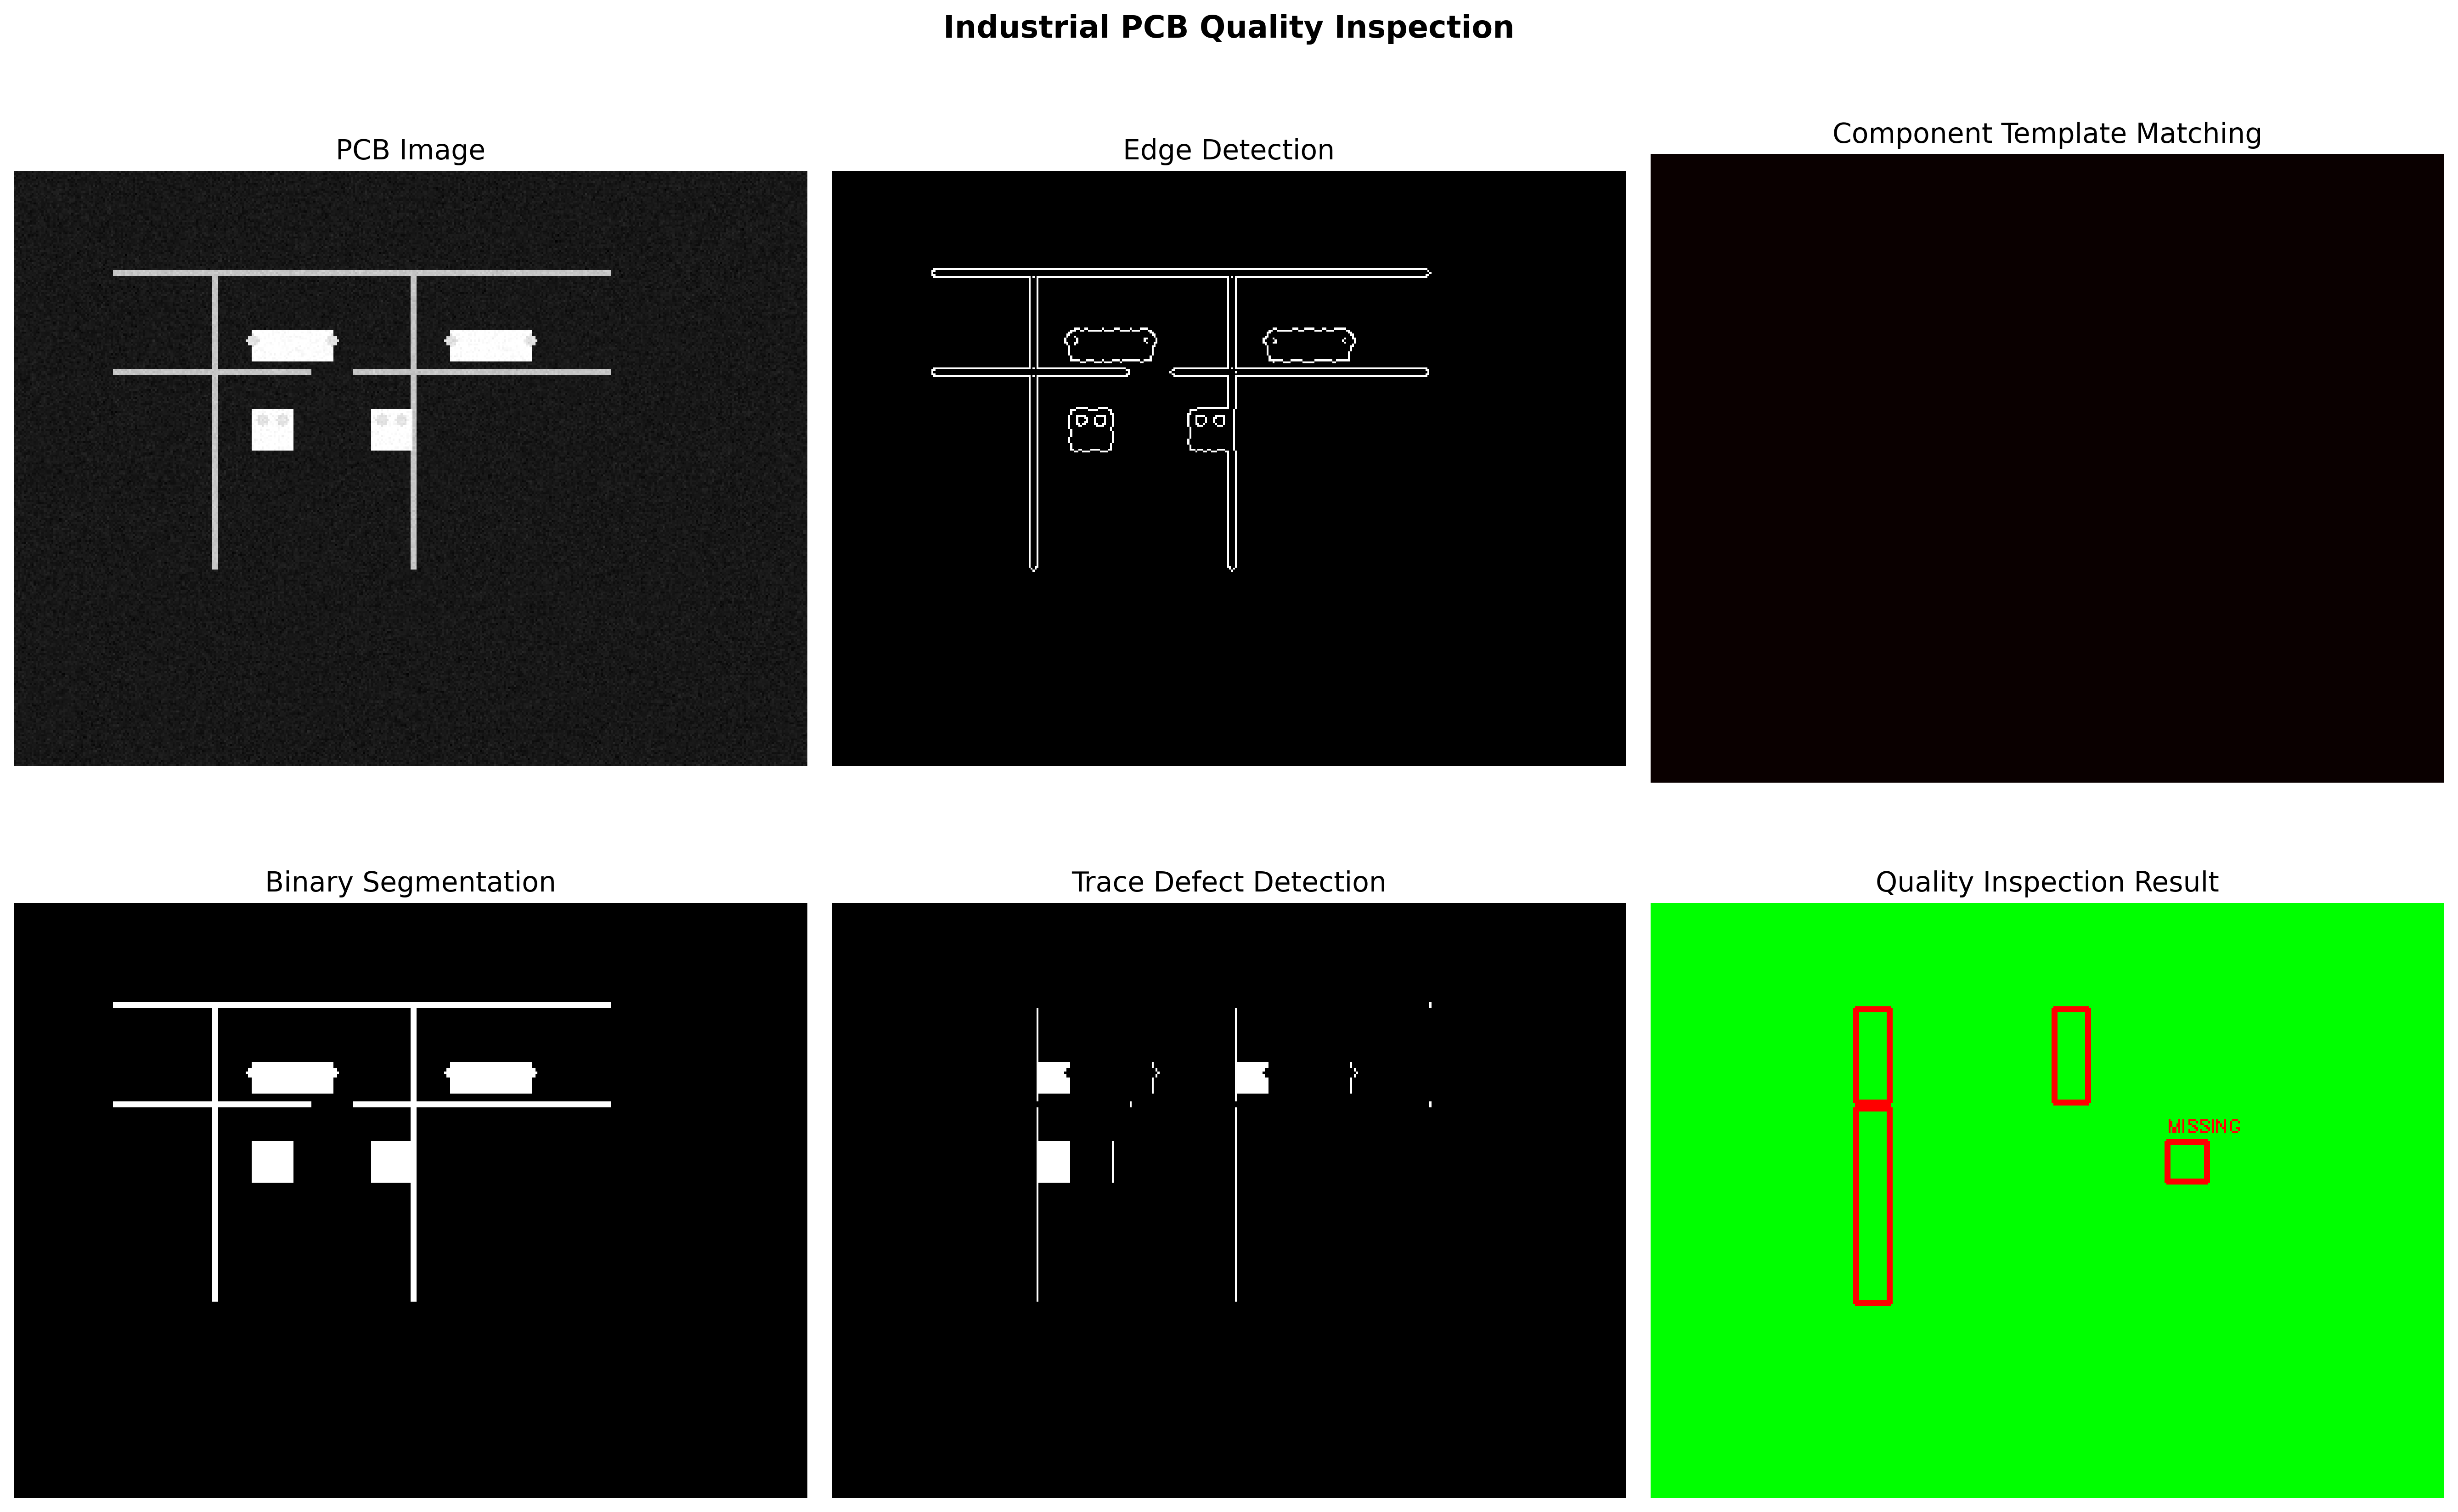
\includegraphics[width=0.75\textwidth,height=0.55\textheight,keepaspectratio]{../figures/industrial_inspection.png}
    \end{center}

    \textbf{Inspection Tasks:}
    \begin{itemize}
        \item Defect detection
        \item Component verification
        \item Assembly validation
        \item Quality assessment
    \end{itemize}
\end{frame}

\begin{frame}{Biometric Analysis}
    \begin{center}
        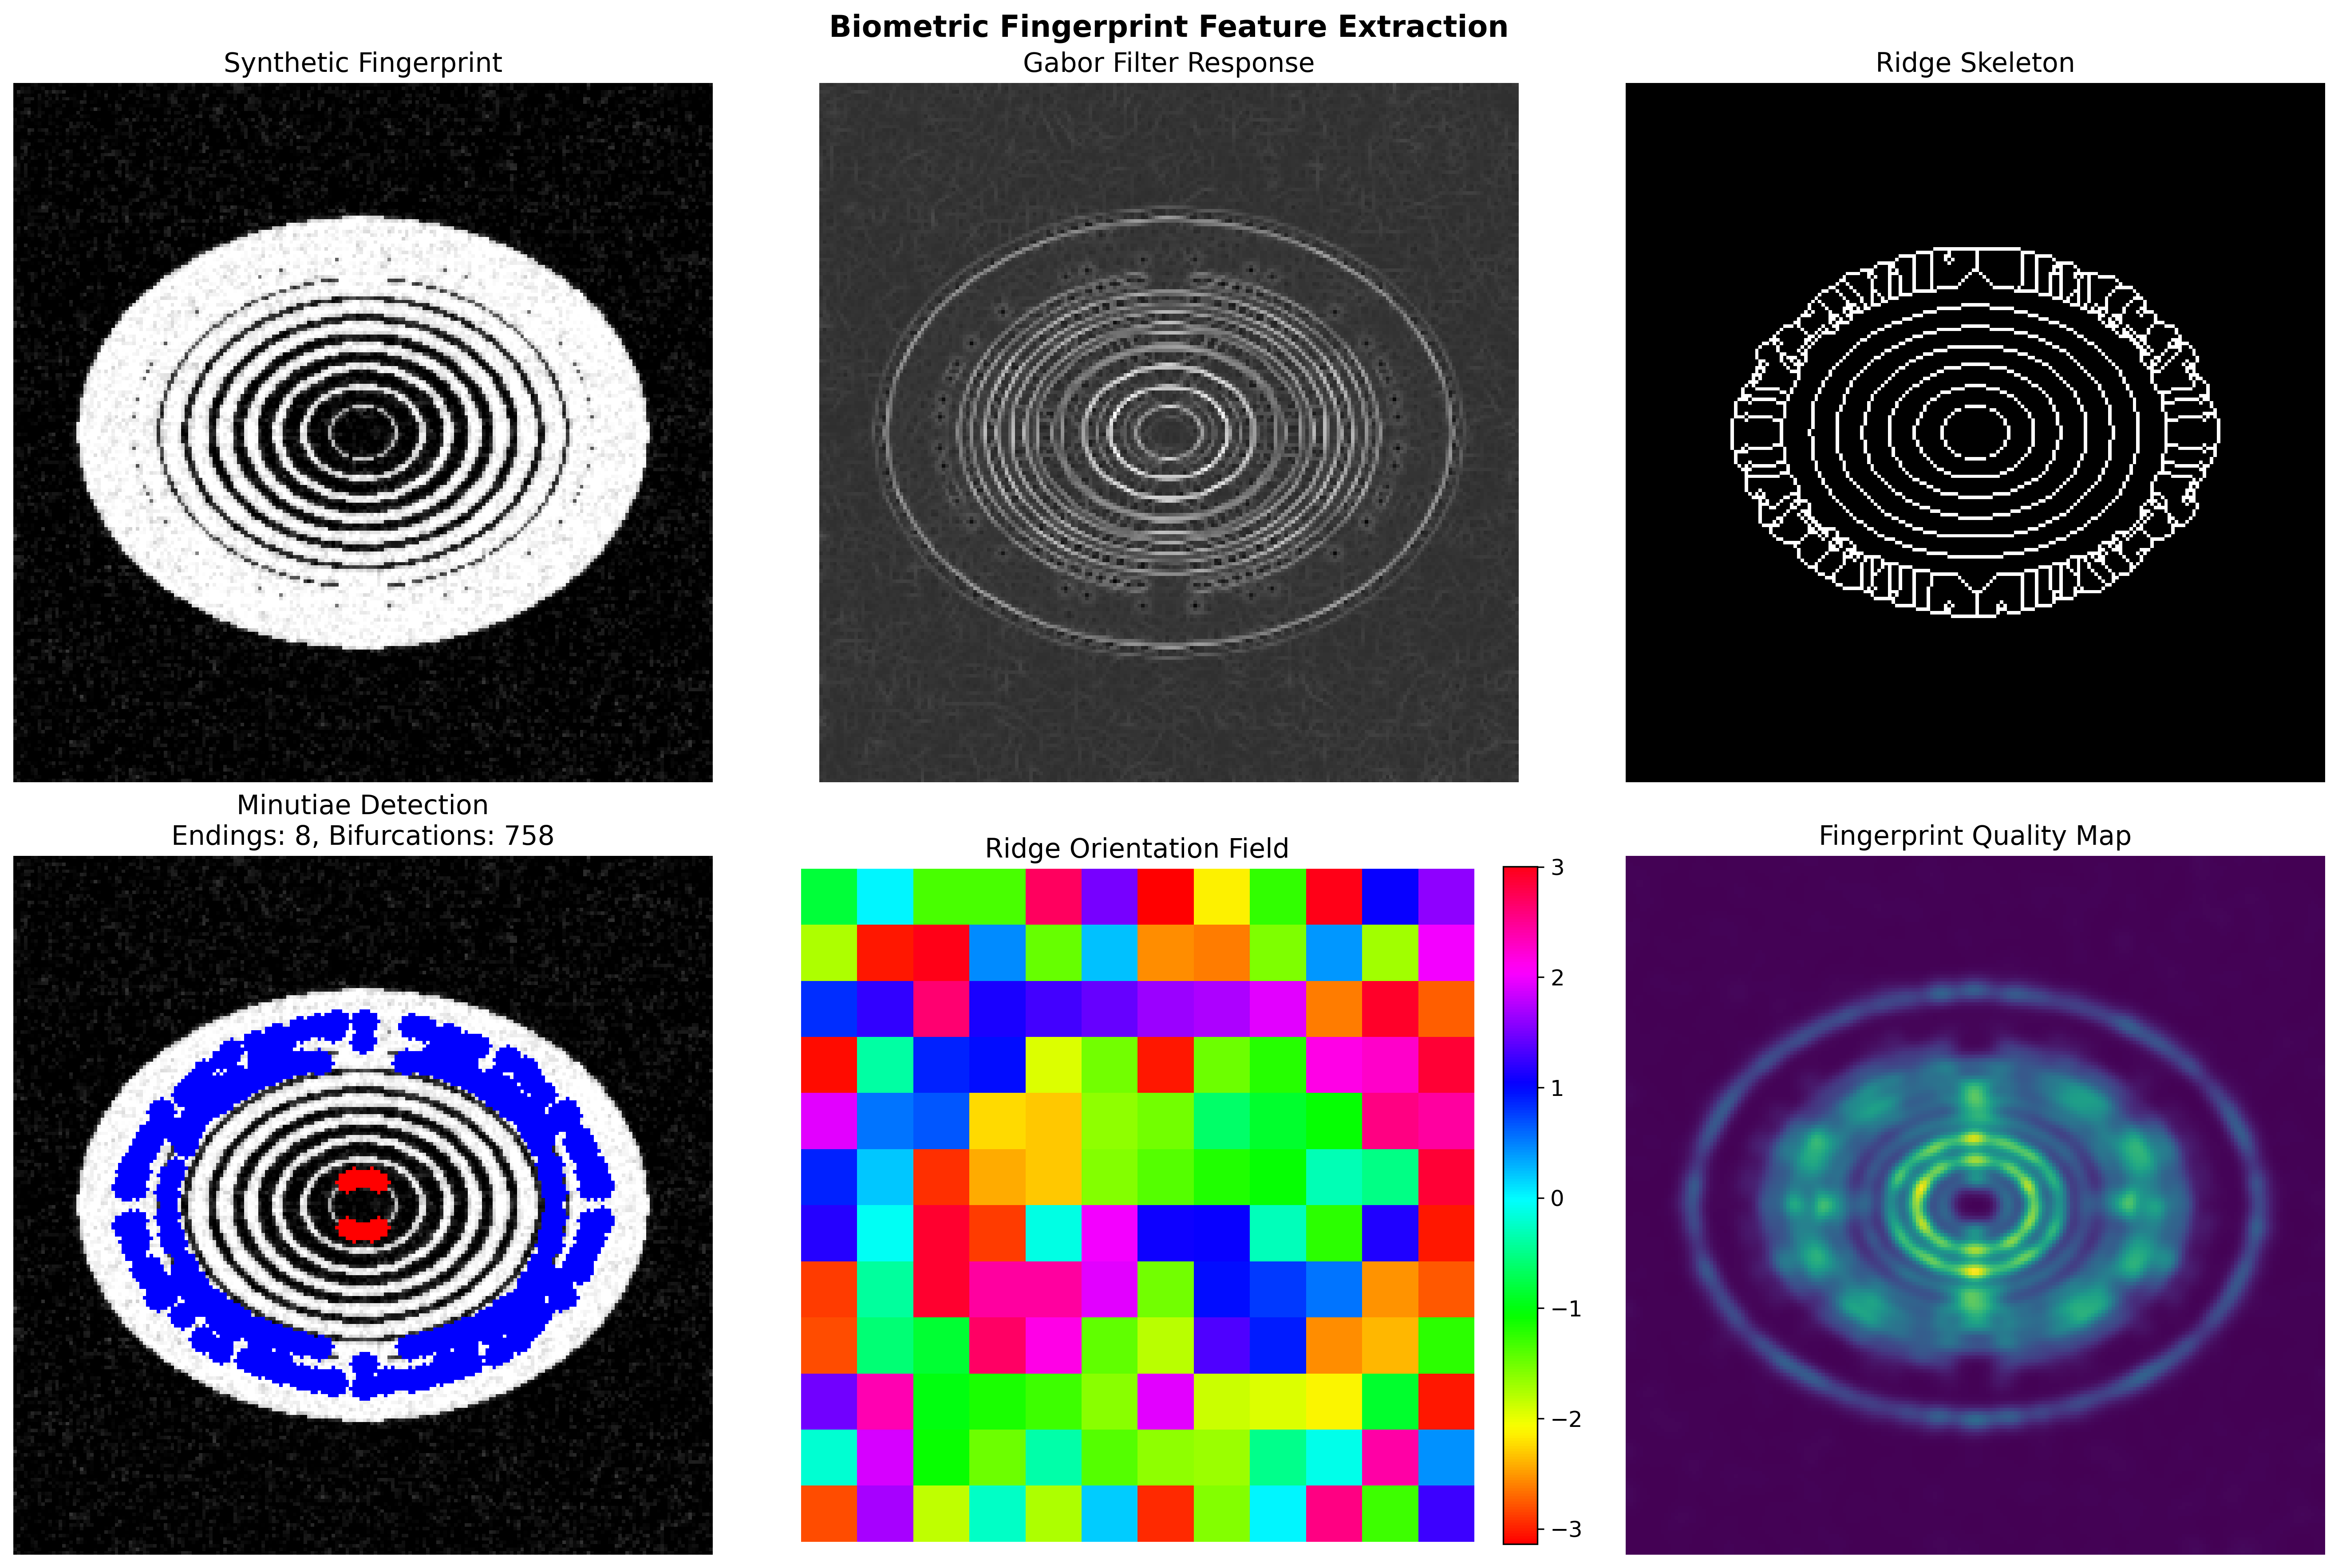
\includegraphics[width=0.75\textwidth,height=0.55\textheight,keepaspectratio]{../figures/biometric_analysis.png}
    \end{center}

    \textbf{Fingerprint Features:}
    \begin{itemize}
        \item Ridge patterns
        \item Minutiae points
        \item Orientation fields
        \item Quality assessment
    \end{itemize}
\end{frame}

\begin{frame}{Autonomous Vehicle Vision}
    \begin{center}
        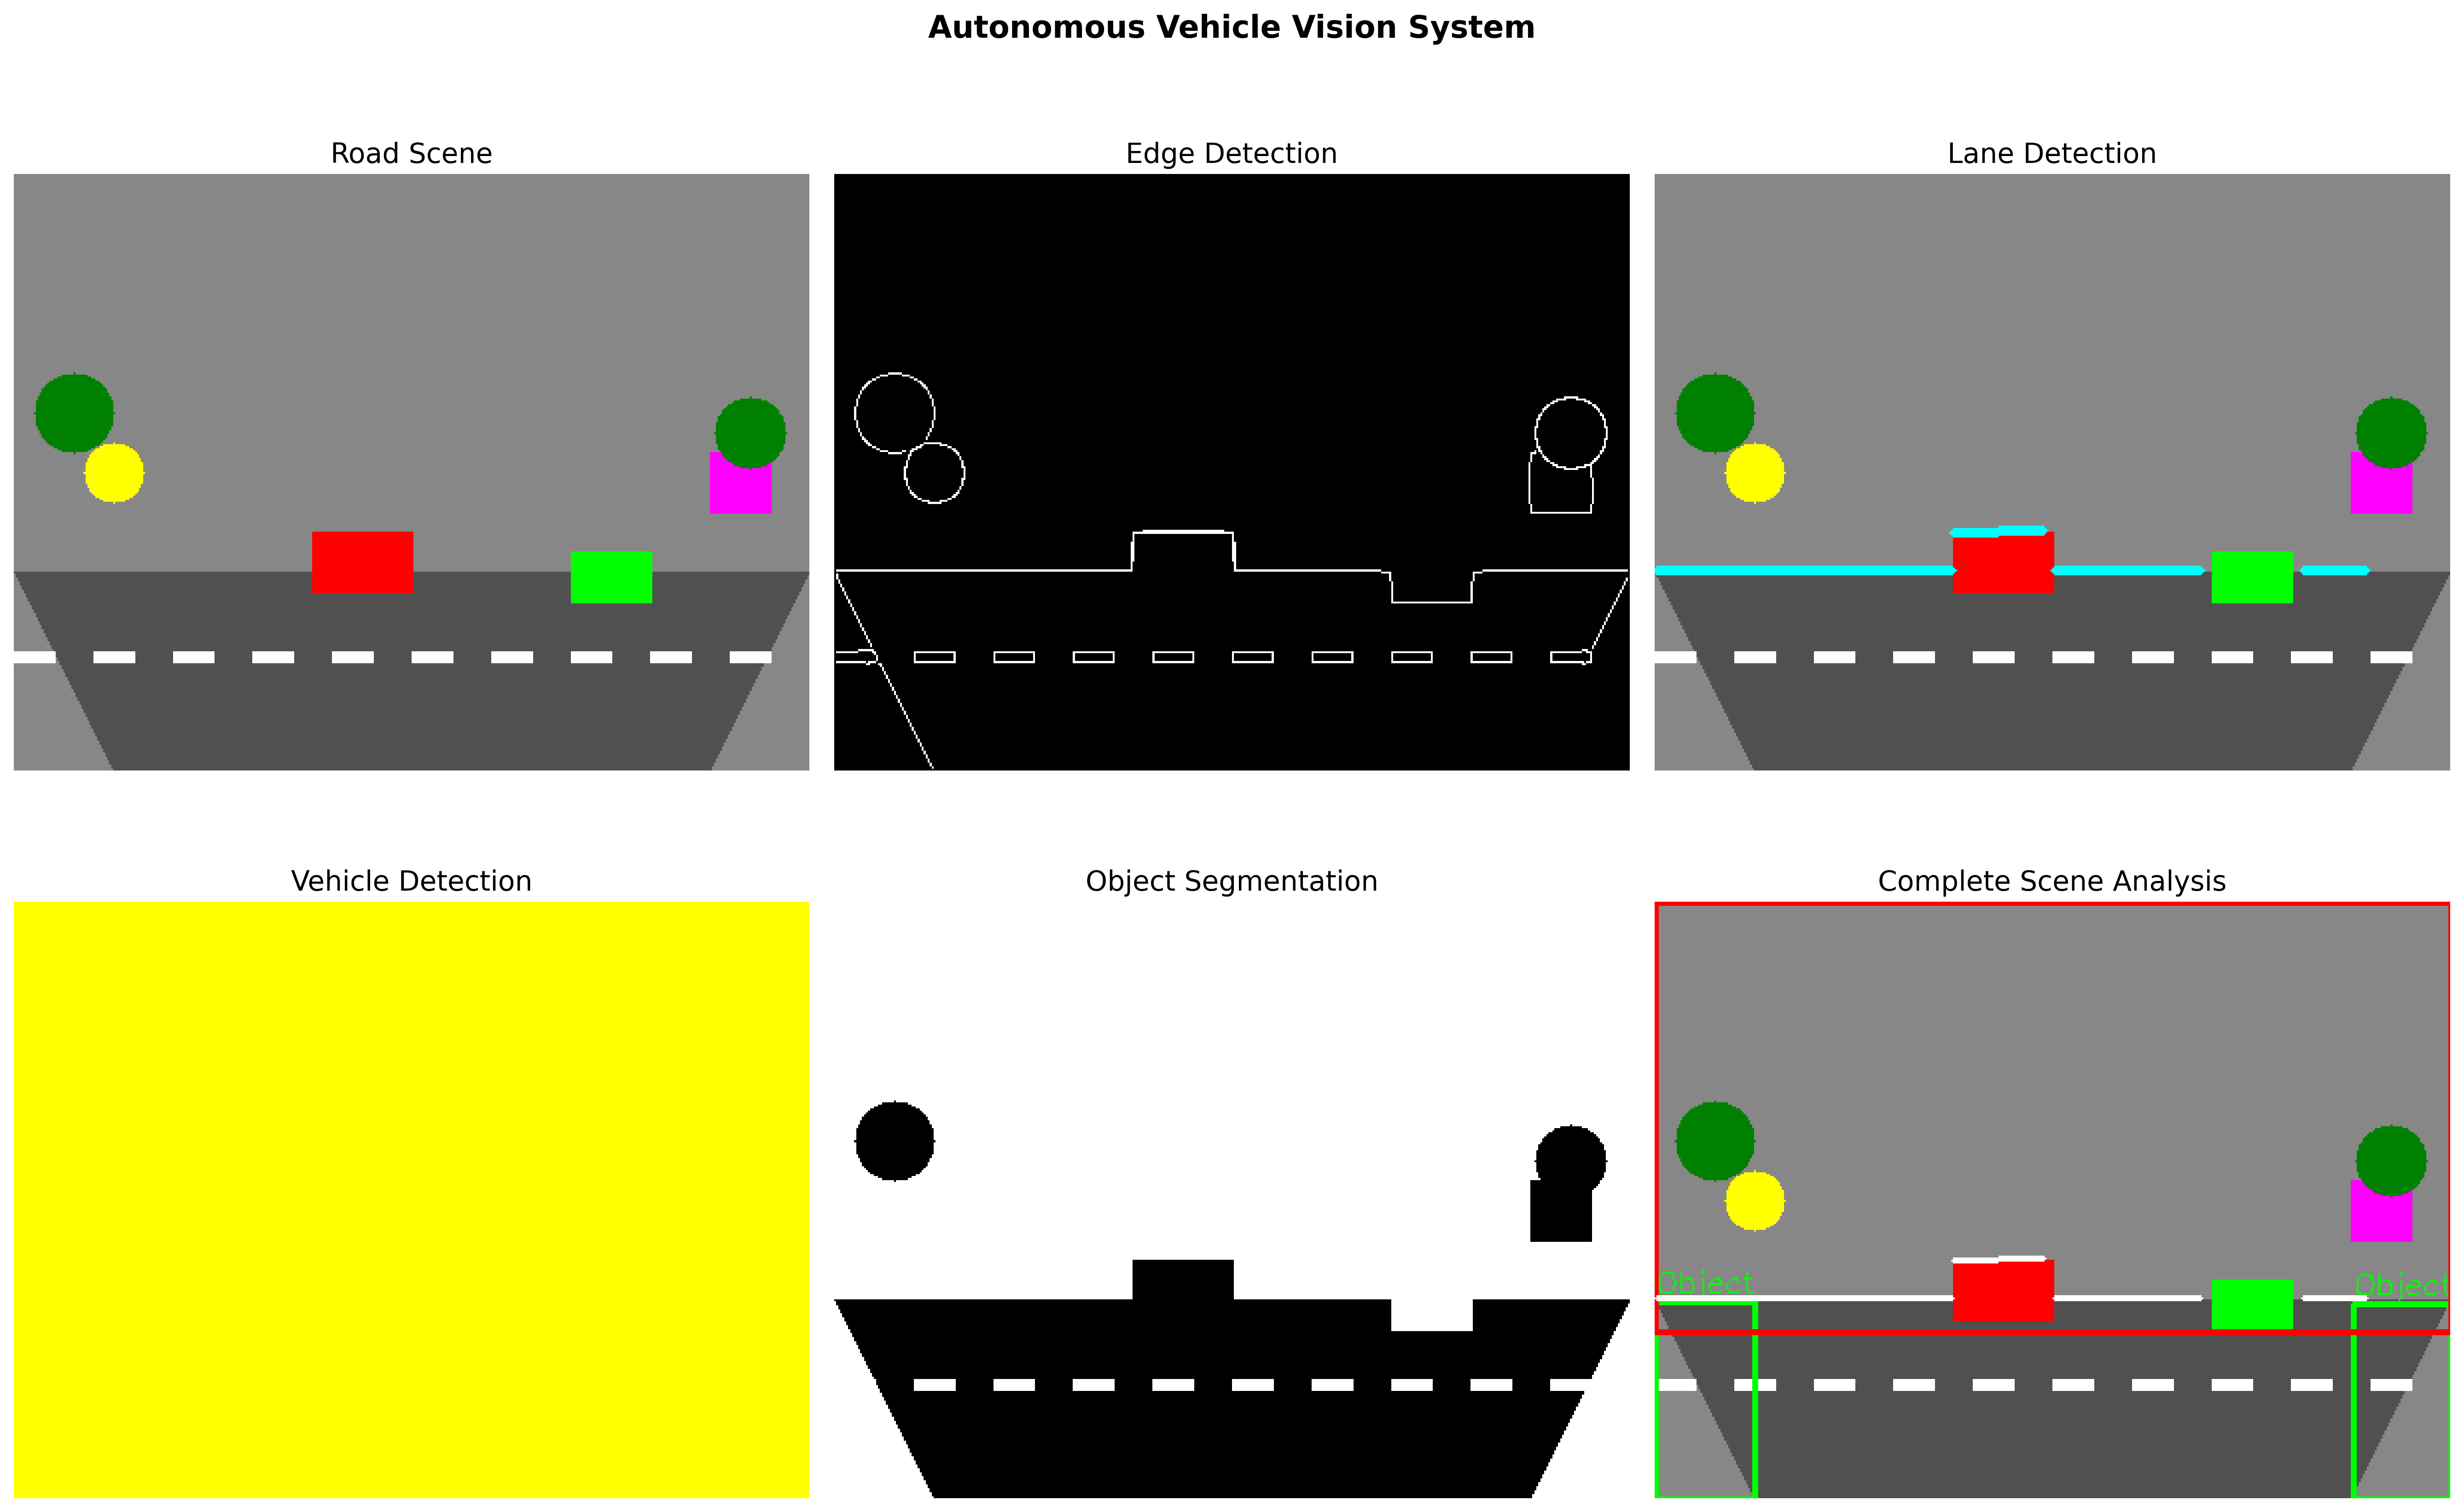
\includegraphics[width=0.75\textwidth,height=0.55\textheight,keepaspectratio]{../figures/autonomous_vehicle.png}
    \end{center}

    \textbf{Vision Tasks:}
    \begin{itemize}
        \item Lane detection
        \item Object recognition
        \item Traffic sign detection
        \item Obstacle avoidance
    \end{itemize}
\end{frame}

\begin{frame}{Bag of Visual Words}
    \begin{center}
        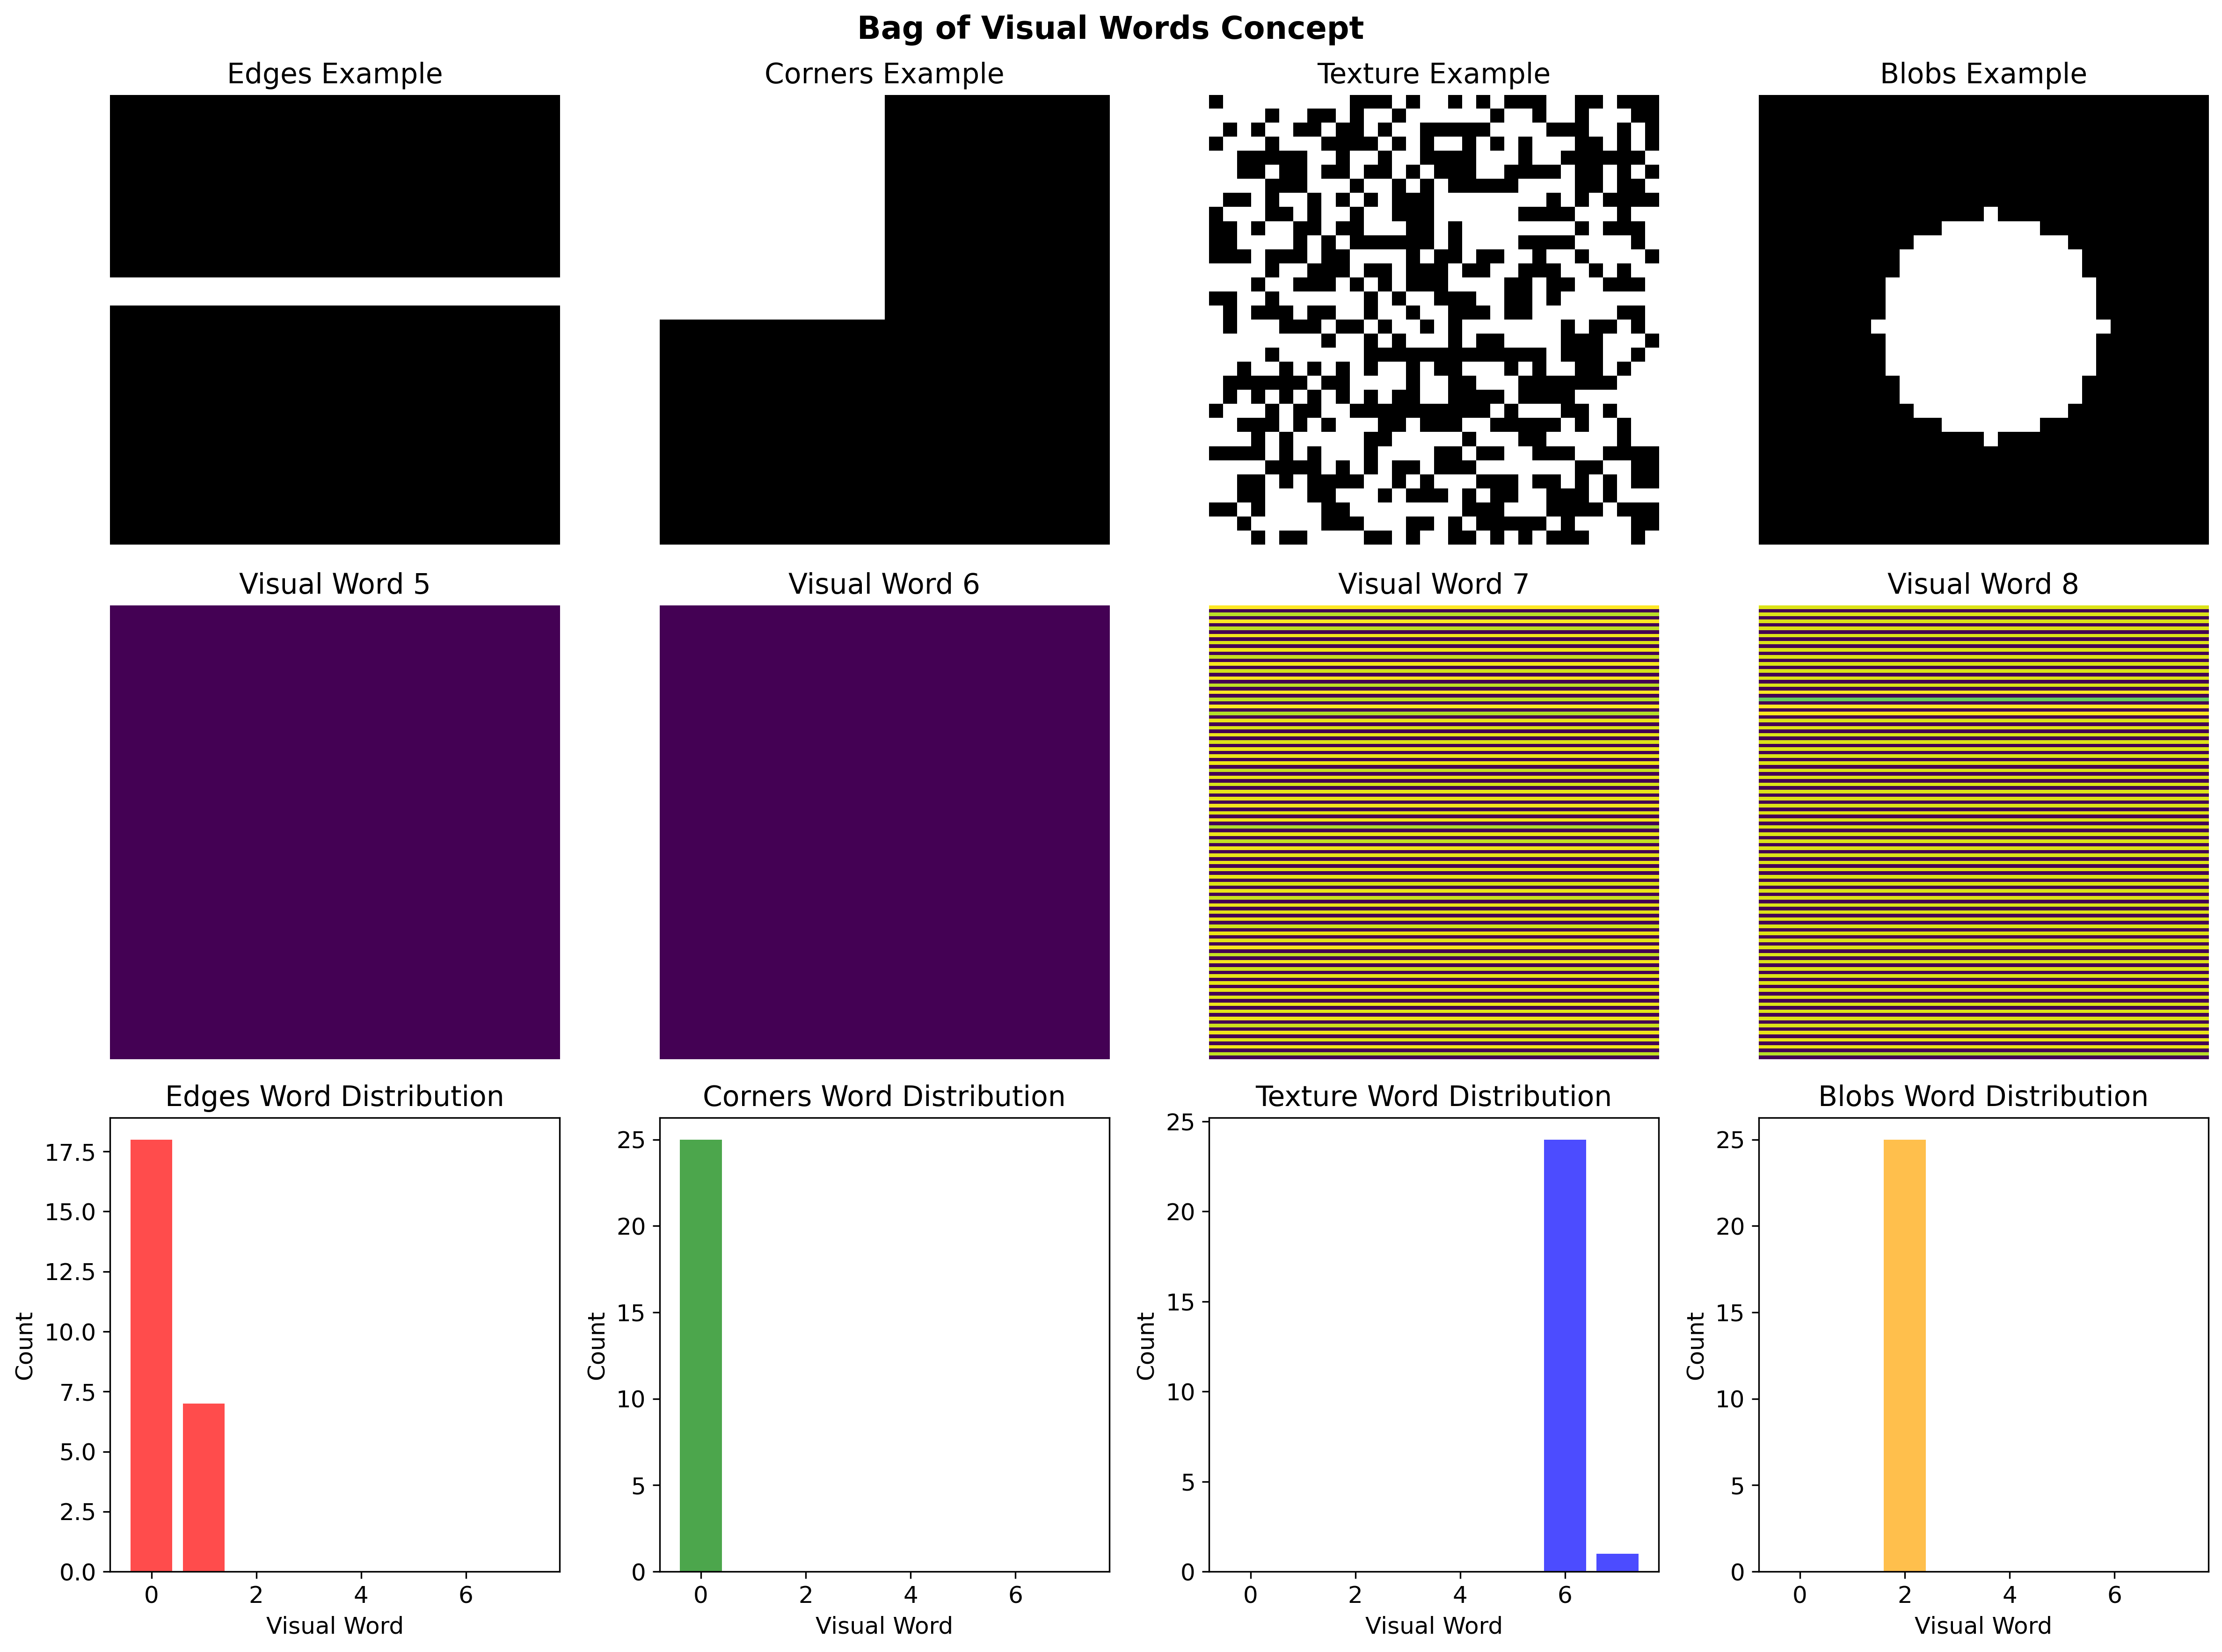
\includegraphics[width=0.75\textwidth,height=0.55\textheight,keepaspectratio]{../figures/bag_of_features.png}
    \end{center}

    \textbf{Concept:}
    \begin{itemize}
        \item Extract local features from training images
        \item Cluster features to create visual vocabulary
        \item Represent images as histograms of visual words
        \item Enable image classification and retrieval
    \end{itemize}
\end{frame}

% Best Practices Section
\section{Best Practices and Guidelines}

\begin{frame}{Feature Selection Guidelines}
    \begin{columns}[c]
        \begin{column}{0.5\textwidth}
            \textbf{Choose Features Based On:}
            \begin{itemize}
                \item Application requirements
                \item Computational constraints
                \item Expected transformations
                \item Illumination conditions
                \item Noise characteristics
            \end{itemize}
        \end{column}
        \begin{column}{0.5\textwidth}
            \textbf{Performance Factors:}
            \begin{itemize}
                \item Repeatability
                \item Distinctiveness
                \item Robustness
                \item Efficiency
                \item Accuracy
            \end{itemize}
        \end{column}
    \end{columns}

    \begin{alertblock}{Key Principle}
        The choice of feature extraction method should align with the specific requirements and constraints of your application.
    \end{alertblock}
\end{frame}

\begin{frame}{Common Pitfalls and Solutions}
    \begin{columns}[c]
        \begin{column}{0.5\textwidth}
            \textbf{Common Problems:}
            \begin{itemize}
                \item Over-sensitive to noise
                \item Poor scale invariance
                \item Computational bottlenecks
                \item Inappropriate feature choice
                \item Insufficient preprocessing
            \end{itemize}
        \end{column}
        \begin{column}{0.5\textwidth}
            \textbf{Solutions:}
            \begin{itemize}
                \item Apply proper smoothing
                \item Use multi-scale approaches
                \item Optimize algorithms
                \item Validate feature selection
                \item Implement robust preprocessing
            \end{itemize}
        \end{column}
    \end{columns}

    \textbf{Validation Strategy:}
    \begin{itemize}
        \item Test on diverse datasets
        \item Measure performance metrics
        \item Compare multiple methods
        \item Consider computational trade-offs
    \end{itemize}
\end{frame}

\begin{frame}{Feature Evaluation Metrics}
    \textbf{Keypoint Detector Evaluation:}
    \begin{itemize}
        \item \textbf{Repeatability:} Percentage of corresponding keypoints detected
        \item \textbf{Localization accuracy:} Spatial precision of detected points
        \item \textbf{Computational efficiency:} Processing time and memory usage
    \end{itemize}

    \textbf{Descriptor Evaluation:}
    \begin{itemize}
        \item \textbf{Distinctiveness:} Ability to discriminate between features
        \item \textbf{Robustness:} Performance under various transformations
        \item \textbf{Matching accuracy:} Precision and recall of feature matching
    \end{itemize}

    \begin{alertblock}{Benchmark Datasets}
        Use standardized datasets like Oxford Dataset, Mikolajczyk Dataset, or custom validation sets for consistent evaluation.
    \end{alertblock}
\end{frame}

% Advanced Topics Section
\section{Advanced Topics}

\begin{frame}{Modern Deep Learning Approaches}
    \textbf{Deep Feature Extraction:}
    \begin{itemize}
        \item Convolutional Neural Networks (CNNs)
        \item Learned feature representations
        \item End-to-end training
        \item Transfer learning capabilities
    \end{itemize}

    \textbf{Advantages over Traditional Methods:}
    \begin{itemize}
        \item Automatic feature learning
        \item Better generalization
        \item State-of-the-art performance
        \item Task-specific optimization
    \end{itemize}

    \textbf{Popular Architectures:}
    \begin{itemize}
        \item ResNet, VGG for general features
        \item SuperPoint for keypoint detection
        \item LoFTR for feature matching
    \end{itemize}
\end{frame}

\begin{frame}{Multi-Scale Feature Analysis}
    \textbf{Scale-Space Theory:}
    \begin{align}
        L(x,y,\sigma) &= G(x,y,\sigma) * I(x,y) \\
        G(x,y,\sigma) &= \frac{1}{2\pi\sigma^2} e^{-\frac{x^2+y^2}{2\sigma^2}}
    \end{align}

    \textbf{Applications:}
    \begin{itemize}
        \item Object detection at multiple scales
        \item Hierarchical image analysis
        \item Feature pyramid networks
        \item Multi-resolution processing
    \end{itemize}

    \textbf{Benefits:}
    \begin{itemize}
        \item Scale invariance
        \item Robust feature detection
        \item Comprehensive image analysis
    \end{itemize}
\end{frame}

\begin{frame}{Real-Time Considerations}
    \textbf{Optimization Strategies:}
    \begin{itemize}
        \item Algorithm selection for speed
        \item Hardware acceleration (GPU, FPGA)
        \item Parallel processing techniques
        \item Approximation methods
    \end{itemize}

    \textbf{Trade-offs:}
    \begin{columns}[c]
        \begin{column}{0.5\textwidth}
            \textbf{Speed vs. Accuracy:}
            \begin{itemize}
                \item FAST vs. SIFT
                \item ORB vs. SURF
                \item Binary vs. float descriptors
            \end{itemize}
        \end{column}
        \begin{column}{0.5\textwidth}
            \textbf{Memory vs. Performance:}
            \begin{itemize}
                \item Descriptor size
                \item Feature density
                \item Storage requirements
            \end{itemize}
        \end{column}
    \end{columns}
\end{frame}

% Summary Section
\section{Summary and Future Directions}

\begin{frame}{Key Takeaways}
    \textbf{Feature Extraction Fundamentals:}
    \begin{itemize}
        \item Edge detection forms the foundation of many computer vision tasks
        \item Local features provide robust image representation
        \item Choice of method depends on application requirements
    \end{itemize}

    \textbf{Important Methods Covered:}
    \begin{itemize}
        \item Gradient operators (Sobel, Prewitt, Roberts)
        \item Advanced edge detection (Canny)
        \item Geometric features (Hough transform)
        \item Texture analysis (LBP, Gabor)
        \item Modern descriptors (SIFT, ORB, HOG)
    \end{itemize}

    \textbf{Practical Applications:}
    \begin{itemize}
        \item Document analysis and OCR
        \item Medical image processing
        \item Industrial quality control
        \item Biometric systems
        \item Autonomous vehicles
    \end{itemize}
\end{frame}

\begin{frame}{Future Directions}
    \textbf{Emerging Trends:}
    \begin{itemize}
        \item Deep learning-based feature extraction
        \item Self-supervised learning methods
        \item Attention mechanisms in feature detection
        \item Neural architecture search for optimal features
    \end{itemize}

    \textbf{Research Challenges:}
    \begin{itemize}
        \item Improving robustness to extreme conditions
        \item Reducing computational requirements
        \item Enhancing interpretability of learned features
        \item Cross-domain feature transfer
    \end{itemize}

    \textbf{Applications on the Horizon:}
    \begin{itemize}
        \item Augmented reality
        \item Advanced medical diagnostics
        \item Smart manufacturing
        \item Environmental monitoring
    \end{itemize}
\end{frame}

\begin{frame}{Next Steps in Learning}
    \textbf{Recommended Practice:}
    \begin{itemize}
        \item Implement basic edge detectors from scratch
        \item Experiment with different feature descriptors
        \item Build a simple object recognition system
        \item Compare performance on various datasets
    \end{itemize}

    \textbf{Further Study:}
    \begin{itemize}
        \item Machine learning for computer vision
        \item 3D feature extraction and matching
        \item Video analysis and temporal features
        \item Deep learning architectures
    \end{itemize}

    \begin{alertblock}{Remember}
        Feature extraction is both an art and a science - understanding the theoretical foundations while gaining practical experience is key to mastering this field.
    \end{alertblock}
\end{frame}

\begin{frame}{}
    \begin{center}
        \Huge{Thank You!}

        \vspace{1cm}

        \Large{Questions and Discussion}

        \vspace{0.5cm}

        \normalsize{
            CMSC 178IP - Digital Image Processing \\
            University of the Philippines - Cebu
        }
    \end{center}
\end{frame}

\end{document}